\chapter{Modelling and Analysis -- From Data to Epicycles}
\label{chap:modelling-analysis}
\markboth{Modelling and Analysis -- From Data to Epicycles}{Modelling and Analysis -- From Data to Epicycles}

\begin{remark}[Periodicity decision for the target of this chapter (citation)]\label{rem:modelling_ps_hook}
When this chapter decides whether a research target is periodic, determines its period type, or seeks its minimal positive period, reference is always made to the `Periodic Systems' chapter:
for the periodicity criterion see \cref{thm:ps_periodicity_decision},
for the discrimination of period types see \cref{def:ps_period_type}, \cref{prop:ps_type_discrimination},
for the search for the minimal positive period see \cref{def:ps_minimal_period_algorithm}, \cref{thm:ps_minimal_period_correctness},
and for the construction of period series and epicycle groups from data see \cref{thm:ps_series_reconstruction}, \cref{def:ps_epicycle_group}.
\end{remark}

\begin{remark}[Position of this chapter: the methodological hinge from data to epicycles]\label{rem:modelling_analysis_positioning}
This chapter establishes the \textbf{unified methodological framework} of periodicity mathematics---from the modelling of real-world problems, data acquisition, periodicity analysis and signal processing through to model evaluation, ultimately reducing to the epicycle model and its complex-valued function implementation. This chapter is the \textbf{bridge chapter} connecting the theoretical system of periodicity mathematics (the `Series and Convolution', `Harmonic Analysis' and `Periodic Systems' chapters) and the various application domains (astronomy, calendars, geography, biology, psychology, economics, politics, algorithms and agents).

The core methodological procedure is:
\[
\boxed{\text{Modelling}} \to \boxed{\text{Data}} \to \boxed{\text{Analysis}} \to \boxed{\text{Processing}} \to \boxed{\text{Evaluation}} \to \boxed{\text{Period}} \to \boxed{\text{Epicycle}} \to \boxed{\text{Waveform}}
\]
Every step uses a core tool of periodicity mathematics: modelling uses symmetry and constraint relations; data acquisition uses the theory of dynamic sampling (\cref{def:dynamic_sampling}); analysis uses periodic convolution (\cref{def:periodic_convolution}) and the similarity/trend lineage (\cref{def:similarity_essence,def:tendency}); processing uses window functions (\cref{def:window_function}) and derivative--integral descent optimisation (\cref{def:kdi_definition}); evaluation uses information criteria (AIC/BIC); period identification uses nested epicycle generation (\cref{def:epicycle_nesting_rule}); and the Waveform, as a complex-valued function, uses the complex exponential activation function (\cref{def:epicycle-activation}).

\textbf{The distinctive contribution of this chapter}: the methodological framework above is expressed in two ways at once, as a \textbf{mathematical statement} and as \textbf{programming modelling (UML/diagrams)}. The mathematical statement provides rigorous theorems and proofs; the programming modelling provides an implementable class system, data flow, interaction sequence and business process. Together they constitute the complete expression of the methodology of this chapter.

\textbf{Guide to the seven themes of this chapter}: translation---the advancement of the time series in data acquisition (\cref{def:data_acquisition}) and the time-translation invariance of the Waveform (\cref{prop:waveform_properties}); scaling---the complexity penalty of BIC (\cref{ch34_pipeline_closure}) and multi-scale window functions (\cref{def:processing_tools}); rotation---the phase $\phi_k$ of the epicycle model (\cref{def:epicycle_modelling}) and the complex phase representation of the Waveform; balance---the fit--complexity balance of BIC (\cref{prop:bic_balance}) and the uniqueness of the parameters given by the Bohr mean (\cref{ch34_epicycle_properties}); symmetry---the hierarchical symmetry of epicycle nesting; closure---the feedback-iteration closure of the methodological procedure (\cref{ch34_pipeline_closure}) and the closure property of the Functor class (\cref{prop:functor_closure}); period---spectral peak identification (\cref{def:period_identification}) and epicycle parameter estimation (\cref{def:epicycle_modelling}).
\end{remark}

\begin{remark}[The dual-track modelling of this chapter]\label{rem:modelling_dual_track}
This chapter expresses `modelling and analysis' in a \textbf{dual-track} manner:
\begin{enumerate}[label=(\roman*)]
    \item \textbf{The mathematical track}: statements and proofs are given in the strict order of definitions, propositions, lemmas, theorems, corollaries, properties, examples and remarks. The mathematical track is the backbone of this chapter, and every conclusion must be verifiable.
    \item \textbf{The engineering track}: expressed by such visualisation tools as Venn diagrams, Gantt charts, flowcharts, UML diagrams (context diagram, use-case diagram, class diagram, object diagram, sequence diagram), system architecture diagrams, user-story maps, business process models, data flow diagrams and ER diagrams. The engineering track is \textbf{supplementary exposition} of the mathematical track---it introduces no new mathematical content, but only translates the objects, relations and processes of the mathematical track into an implementable engineering language.
\end{enumerate}
The interface convention between the two tracks is: every concept appearing in the engineering track (such as `Waveform', `Epicycle' and `PeriodicSeries') has already been given a rigorous definition in the mathematical track or in an earlier chapter; the diagrams of the engineering track \textbf{constitute no new mathematical assertion}. This convention guarantees that the chapter preserves mathematical rigour without sacrificing engineering implementability.
\end{remark}

\begin{lemma}[Feedback closure of the methodological pipeline]\label{ch34_pipeline_closure}
Let the model class $\mathcal{M} = \{\mathcal{M}_K\}_{K=1}^{K_{\max}}$ be finite, where $K$ is the epicycle order. The evaluation index is BIC:
\[
\operatorname{BIC}(K) = n\ln(\operatorname{RSS}/n) + K\ln n,
\]
where $n$ is the sample size and $\operatorname{RSS}$ is the residual sum of squares. Then the iteration `evaluation $\to$ feedback $\to$ remodelling' decreases strictly in BIC and converges in finitely many steps to the BIC-optimal model over $\mathcal{M}$.
\end{lemma}

\begin{proof}
The feedback rule is: replace $\mathcal{M}_K$ by $\mathcal{M}_{K'}$ only when $\operatorname{BIC}(K') < \operatorname{BIC}(K)$. Hence BIC decreases strictly at each iteration. Since $\mathcal{M}$ is finite ($K \le K_{\max}$), the possible values of BIC are finite, so a strictly decreasing sequence must terminate after finitely many steps at some $K^*$. At that point there is no replaceable model with a smaller BIC, so $\mathcal{M}_{K^*}$ is the BIC-optimal model over $\mathcal{M}$.
\end{proof}

\section{Overview of the methodology: context diagram and master flow diagram}

\subsection{Context diagram: the boundary between the methodology and external systems}

\begin{figure}[htbp]
    \centering
    \adjustbox{max width=\textwidth}{%
    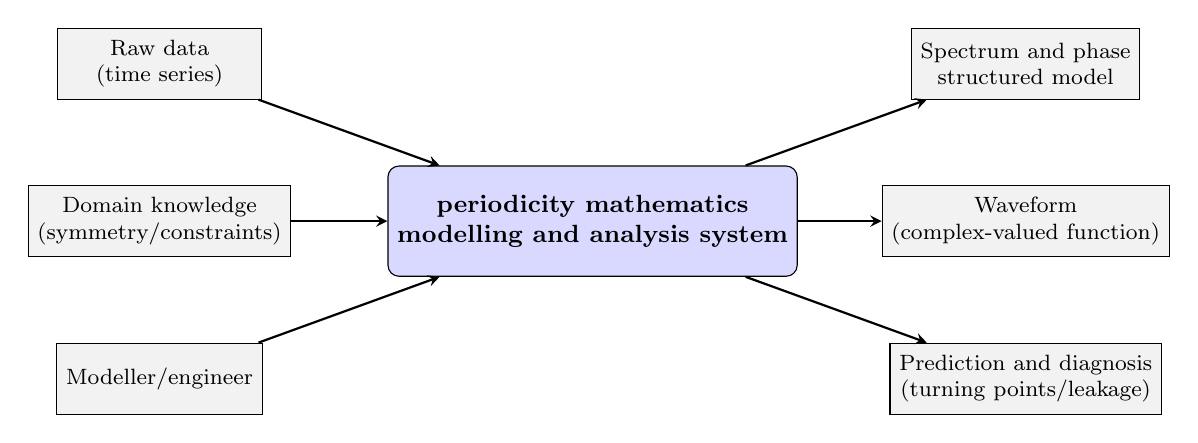
\begin{tikzpicture}[>=stealth,
        sys/.style={draw, rounded corners, fill=blue!15,
                    minimum width=4.2cm, minimum height=1.4cm,
                    align=center, font=\small\bfseries},
        ext/.style={draw, fill=gray!10,
                    minimum width=2.6cm, minimum height=0.9cm,
                    align=center, font=\footnotesize},
        arrow/.style={->, thick, >=stealth}]

        \node[sys] (sys) at (0,0) {periodicity mathematics\\modelling and analysis system};

        \node[ext] (raw)  at (-5.5, 2.0) {Raw data\\(time series)};
        \node[ext] (know) at (-5.5, 0.0) {Domain knowledge\\(symmetry/constraints)};
        \node[ext] (user) at (-5.5,-2.0) {Modeller/engineer};

        \node[ext] (spec) at ( 5.5, 2.0) {Spectrum and phase\\structured model};
        \node[ext] (wf)   at ( 5.5, 0.0) {Waveform\\(complex-valued function)};
        \node[ext] (pred) at ( 5.5,-2.0) {Prediction and diagnosis\\(turning points/leakage)};

        \draw[arrow] (raw)  -- (sys);
        \draw[arrow] (know) -- (sys);
        \draw[arrow] (user) -- (sys);

        \draw[arrow] (sys) -- (spec);
        \draw[arrow] (sys) -- (wf);
        \draw[arrow] (sys) -- (pred);

    \end{tikzpicture}%
    }
    \caption{Context diagram of the periodicity mathematics modelling and analysis system. The inputs are the raw time series, domain knowledge and modeller interaction;
             the outputs are the spectrum and phase structured model, the Waveform complex-valued function representation, and the results of prediction and diagnosis.}
    \label{fig:context_diagram}
\end{figure}

\newpage

\subsection{Master flow diagram}

\begin{figure}[htbp]
    \centering
    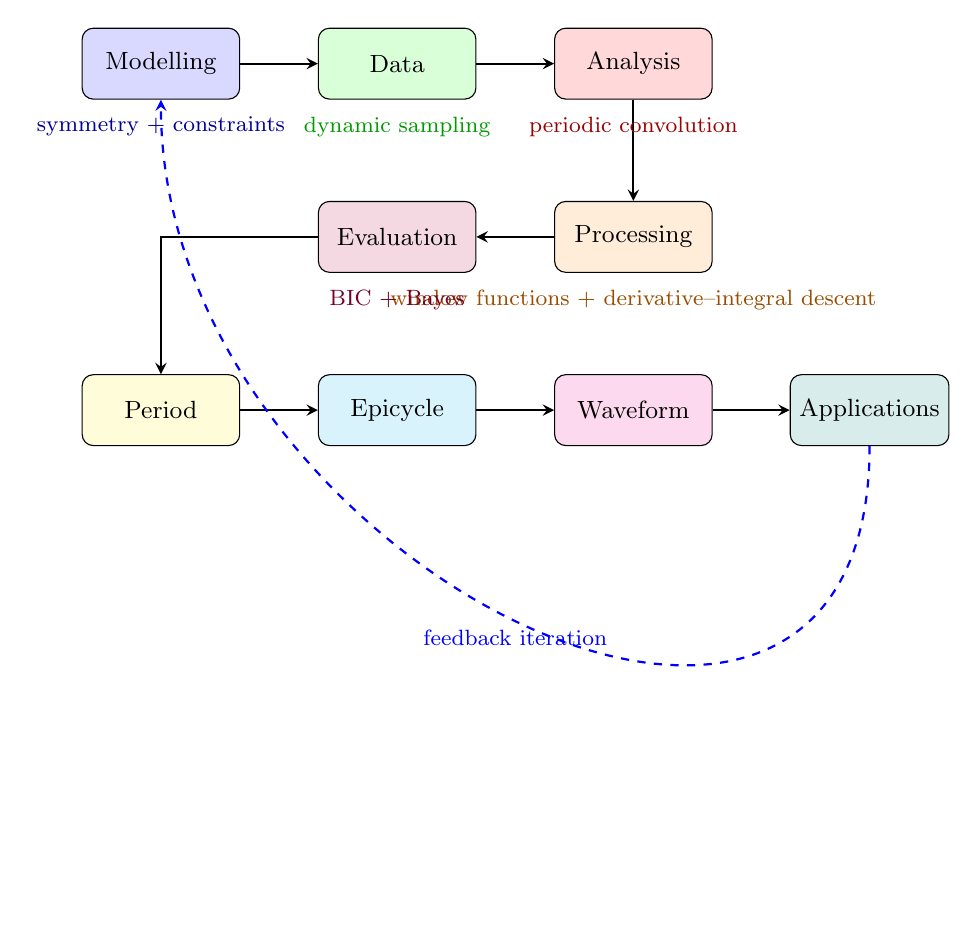
\begin{tikzpicture}[>=stealth,
        box/.style={draw, rounded corners, minimum width=2.0cm, minimum height=0.9cm, align=center, font=\small},
        arrow/.style={->, thick, >=stealth}]
        
        \node[box, fill=blue!15] (model) at (0,0) {Modelling};
        \node[box, fill=green!15] (data) at (3,0) {Data};
        \node[box, fill=red!15] (analysis) at (6,0) {Analysis};
        
        \node[box, fill=orange!15] (processing) at (6,-2.2) {Processing};
        \node[box, fill=purple!15] (evaluation) at (3,-2.2) {Evaluation};
        
        \node[box, fill=yellow!15] (period) at (0,-4.4) {Period};
        \node[box, fill=cyan!15] (epicycle) at (3,-4.4) {Epicycle};
        \node[box, fill=magenta!15] (waveform) at (6,-4.4) {Waveform};
        \node[box, fill=teal!15] (applications) at (9,-4.4) {Applications};
        
        \draw[arrow] (model) -- (data);
        \draw[arrow] (data) -- (analysis);
        \draw[arrow] (analysis) -- (processing);  
        \draw[arrow] (processing) -- (evaluation);  
        \draw[arrow] (evaluation.west) -| (period.north);
        \draw[arrow] (period) -- (epicycle);
        \draw[arrow] (epicycle) -- (waveform);
        \draw[arrow] (waveform) -- (applications);
        
        \draw[arrow, dashed, blue, thick] (applications.south) to[out=-90, in=-90, looseness=1.5]
            node[below, font=\footnotesize] {feedback iteration} (model.south);
        
        \node[font=\footnotesize, text=blue!60!black]   at (0,-0.8) {symmetry + constraints};
        \node[font=\footnotesize, text=green!60!black]  at (3,-0.8) {dynamic sampling};
        \node[font=\footnotesize, text=red!60!black]    at (6,-0.8) {periodic convolution};
        \node[font=\footnotesize, text=orange!60!black] at (6,-3.0) {window functions + derivative--integral descent};
        \node[font=\footnotesize, text=purple!60!black] at (3,-3.0) {BIC + Bayes};
        
    \end{tikzpicture}
    \caption{Master flow diagram of the unified methodology of periodicity mathematics (serpentine loop layout). The first row runs from left to right through modelling, data and analysis;
             the second row runs from right to left through processing and evaluation; the third row runs from left to right through the output structures: period, epicycle, Waveform and applications.
             The dashed arrow denotes the feedback iteration from the applications back to modelling.}
    \label{fig:methodology_main_flow}
\end{figure}

\newpage

\section{Venn diagram of the concept sets}

\begin{figure}[htbp]
    \centering
    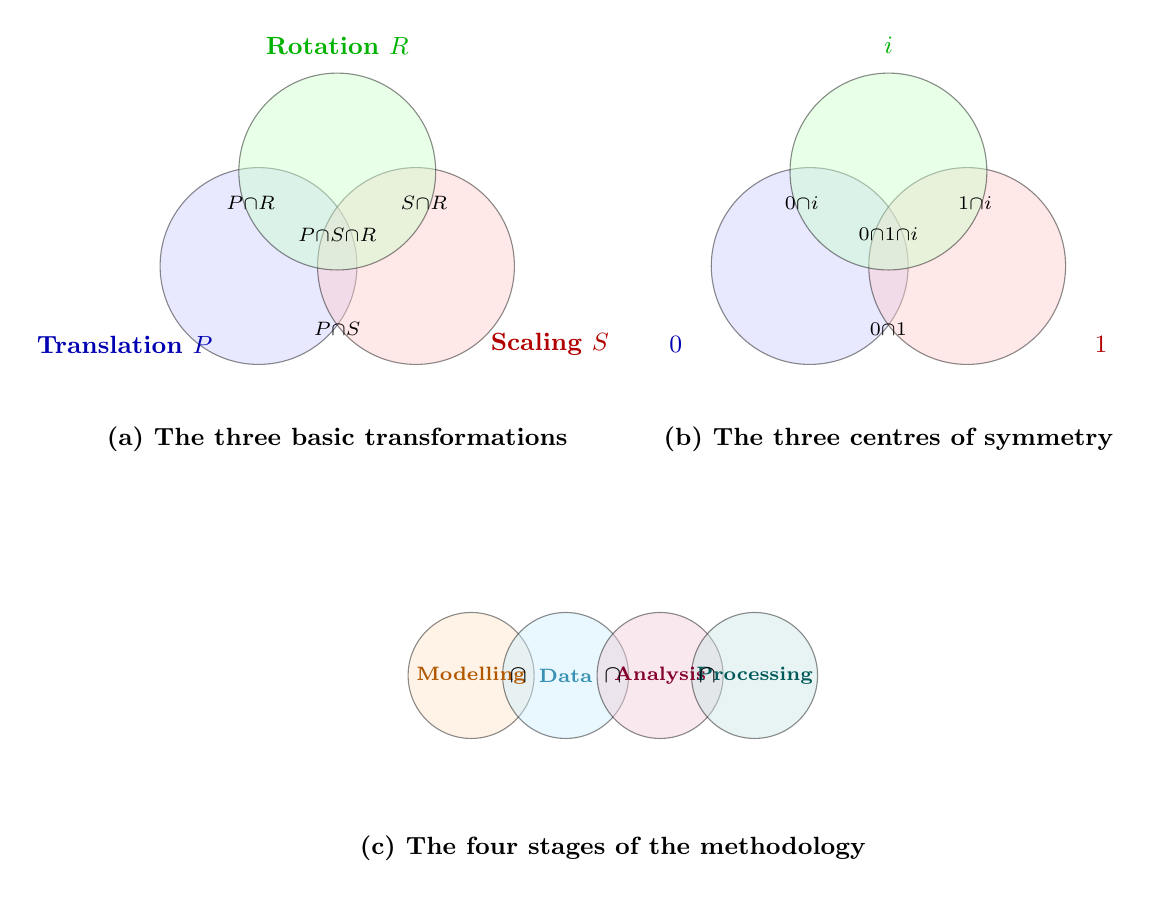
\begin{tikzpicture}[>=stealth, font=\small]

        \begin{scope}
            \draw[fill=blue!20,   opacity=0.45] (-1.0, 0.0) circle (1.25);
            \draw[fill=red!20,    opacity=0.45] ( 1.0, 0.0) circle (1.25);
            \draw[fill=green!20,  opacity=0.45] ( 0.0, 1.2) circle (1.25);

            \node[font=\small\bfseries, blue!70!black]  at (-2.7, -1.0) {Translation $P$};
            \node[font=\small\bfseries, red!70!black]   at ( 2.7, -1.0) {Scaling $S$};
            \node[font=\small\bfseries, green!70!black] at ( 0.0,  2.8) {Rotation $R$};

            \node[font=\scriptsize] at (-1.1,  0.8) {$P{\cap}R$};
            \node[font=\scriptsize] at ( 1.1,  0.8) {$S{\cap}R$};
            \node[font=\scriptsize] at ( 0.0, -0.8) {$P{\cap}S$};
            \node[font=\scriptsize] at ( 0.0,  0.4) {$P{\cap}S{\cap}R$};

            \node[font=\small\bfseries] at (0, -2.2) {(a) The three basic transformations};
        \end{scope}

        \begin{scope}[xshift=7cm]
            \draw[fill=blue!20,   opacity=0.45] (-1.0, 0.0) circle (1.25);
            \draw[fill=red!20,    opacity=0.45] ( 1.0, 0.0) circle (1.25);
            \draw[fill=green!20,  opacity=0.45] ( 0.0, 1.2) circle (1.25);

            \node[font=\small\bfseries, blue!70!black]  at (-2.7, -1.0) {$0$};
            \node[font=\small\bfseries, red!70!black]   at ( 2.7, -1.0) {$1$};
            \node[font=\small\bfseries, green!70!black] at ( 0.0,  2.8) {$i$};

            \node[font=\scriptsize] at (-1.1,  0.8) {$0{\cap}i$};
            \node[font=\scriptsize] at ( 1.1,  0.8) {$1{\cap}i$};
            \node[font=\scriptsize] at ( 0.0, -0.8) {$0{\cap}1$};
            \node[font=\scriptsize] at ( 0.0,  0.4) {$0{\cap}1{\cap}i$};

            \node[font=\small\bfseries] at (0, -2.2) {(b) The three centres of symmetry};
        \end{scope}

        \begin{scope}[yshift=-5.2cm, xshift=3.5cm]
            \draw[fill=orange!20, opacity=0.45] (-1.8, 0) circle (0.8);
            \draw[fill=cyan!20,   opacity=0.45] (-0.6, 0) circle (0.8);
            \draw[fill=purple!20, opacity=0.45] ( 0.6, 0) circle (0.8);
            \draw[fill=teal!20,   opacity=0.45] ( 1.8, 0) circle (0.8);

            \node[font=\scriptsize\bfseries, orange!70!black] at (-1.8, 0) {Modelling};
            \node[font=\scriptsize\bfseries, cyan!70!black]   at (-0.6, 0) {Data};
            \node[font=\scriptsize\bfseries, purple!70!black] at ( 0.6, 0) {Analysis};
            \node[font=\scriptsize\bfseries, teal!70!black]   at ( 1.8, 0) {Processing};

            \node[font=\small] at (-1.2, 0.0) {$\cap$};
            \node[font=\small] at ( 0.0, 0.0) {$\cap$};
            \node[font=\small] at ( 1.2, 0.0) {$\cap$};

            \node[font=\small\bfseries] at (0, -2.2) {(c) The four stages of the methodology};
        \end{scope}

    \end{tikzpicture}
    \caption{Venn diagram of the concept sets. In subfigure (a), $P$ is translation, $S$ is scaling and $R$ is rotation,
             showing the pairwise intersections $P{\cap}S$, $P{\cap}R$ and $S{\cap}R$ of the three basic transformations
             together with the triple intersection $P{\cap}S{\cap}R$;
             subfigure (b) is the overlap of the three centres of symmetry ($0$ for addition, $1$ for multiplication, $i$ for rotation);
             subfigure (c) is the covering relation of adjacent stages among the four stages of the methodology (modelling, data, analysis, processing).
             The Venn diagram displays the coincidences and complementarities among concepts and constitutes no new mathematical assertion.}
    \label{fig:venn_concepts}
\end{figure}

\newpage

\section{Gantt chart of the modelling workflow}

\begin{figure}[htbp]
    \centering
    \begin{tikzpicture}[>=stealth, xscale=1.0, yscale=0.75]
        \draw[->] (0,0) -- (11,0) node[right, font=\footnotesize] {relative workload};
        \foreach \x in {1,2,...,10} {
            \draw[gray!40] (\x,0) -- (\x,6.6);
            \node[font=\tiny, below] at (\x,0) {\x};
        }
        
        \filldraw[fill=blue!60, draw=blue!80] (0,6) rectangle (1.2,6.7);
        \node[font=\footnotesize, right] at (1.2,6.35) {Modelling: identify the transformation group and the invariants};
        
        \filldraw[fill=green!60, draw=green!80] (1.2,5) rectangle (2.5,5.7);
        \node[font=\footnotesize, right] at (2.5,5.35) {Data: dynamic sampling and preprocessing};
        
        \filldraw[fill=red!60, draw=red!80] (2.5,4) rectangle (5.0,4.7);
        \node[font=\footnotesize, right] at (5.0,4.35) {Analysis: FFT/periodic convolution/similarity};
        
        \filldraw[fill=orange!60, draw=orange!80] (5.0,3) rectangle (7.5,3.7);
        \node[font=\footnotesize, right] at (7.5,3.35) {Processing: window-function smoothing and turning-point detection};
        
        \filldraw[fill=purple!60, draw=purple!80] (7.5,2) rectangle (9.0,2.7);
        \node[font=\footnotesize, right] at (9.0,2.35) {Evaluation: BIC/AIC model selection};
        
        \filldraw[fill=cyan!60, draw=cyan!80] (9.0,1) rectangle (10.0,1.7);
        \node[font=\footnotesize, right] at (10.0,1.35) {Output: Waveform};
        
        \draw[->, thick, gray] (1.2,6.35) -- (1.2,5.35);
        \draw[->, thick, gray] (2.5,5.35) -- (2.5,4.35);
        \draw[->, thick, gray] (5.0,4.35) -- (5.0,3.35);
        \draw[->, thick, gray] (7.5,3.35) -- (7.5,2.35);
        \draw[->, thick, gray] (9.0,2.35) -- (9.0,1.35);
        
        \draw[->, thick, dashed, blue] (10.0,1.0) to[bend right=20] (0.3,6.3);
        \node[font=\footnotesize, blue!70!black] at (5,-0.9) {feedback iteration (\cref{ch34_pipeline_closure})};
    \end{tikzpicture}
    \caption{Gantt chart of the modelling workflow. The horizontal axis is the \textbf{relative workload} (a dimensionless unit) and does not represent actual calendar time; the vertical direction is the sequence of tasks. The feedback iteration is guaranteed to converge in finitely many steps by \cref{ch34_pipeline_closure}.}
    \label{fig:gantt_workflow}
\end{figure}

\newpage

\section{Use-case diagram}

\begin{figure}[htbp]
    \centering
    \begin{tikzpicture}[
        >=stealth,
        usecase/.style={draw, ellipse, fill=blue!10, minimum width=2.8cm,
                        minimum height=0.85cm, align=center, font=\footnotesize},
        stickman/.pic={
            \draw[thick] (0,0.25) circle (0.15);
            \draw[thick] (-0.2,-0.05) -- (0.2,-0.05);
            \draw[thick] (0,0.10) -- (0,-0.30);
            \draw[thick] (-0.20,-0.55) -- (0,-0.30) -- (0.20,-0.55);
        }
    ]

        \coordinate (analyst)  at (-5, 3);
        \pic at (analyst)  {stickman};
        \node[font=\footnotesize] at (-5, 2.3) {Modeller};

        \coordinate (engineer) at (-5, 0);
        \pic at (engineer) {stickman};
        \node[font=\footnotesize] at (-5, -0.7) {Engineer};

        \coordinate (data)     at (-5, -3);
        \pic at (data)     {stickman};
        \node[font=\footnotesize] at (-5, -3.7) {Data source};

        \draw[thick, rounded corners] (-3, -4.2) rectangle (4, 4.2);
        \node[font=\small\bfseries] at (0.5, 3.9) {Modelling and analysis system};

        \node[usecase] (uc1) at (0.5,  3.0) {Identify the transformation group};
        \node[usecase] (uc2) at (0.5,  2.0) {Fit epicycle parameters};
        \node[usecase] (uc3) at (0.5,  1.0) {Construct the Waveform};
        \node[usecase] (uc4) at (0.5,  0.0) {Turning-point and refraction-rate diagnosis};
        \node[usecase] (uc5) at (0.5, -1.0) {Phase-coupling network analysis};
        \node[usecase] (uc6) at (0.5, -2.0) {Model selection (BIC/AIC)};
        \node[usecase] (uc7) at (0.5, -3.0) {Sampling and resampling};

        \draw (analyst)  -- (uc1);
        \draw (analyst)  -- (uc2);
        \draw (analyst)  -- (uc4);
        \draw (engineer) -- (uc3);
        \draw (engineer) -- (uc5);
        \draw (engineer) -- (uc6);
        \draw (data)     -- (uc7);

        \draw[dashed, ->] (uc3) -- node[right, font=\tiny] {$\ll$include$\gg$} (uc2);
        \draw[dashed, ->] (uc2) -- node[right, font=\tiny] {$\ll$include$\gg$} (uc7);

    \end{tikzpicture}
    \caption{Use-case diagram of the modelling and analysis system. There are three actors: the modeller, the engineer and the data source.
             The core use cases include identifying the transformation group, fitting epicycle parameters, constructing the Waveform,
             turning-point diagnosis, phase-coupling analysis, model selection, and sampling and resampling.}
    \label{fig:use_case}
\end{figure}

\newpage

\section{User-story map}

\begin{figure}[htbp]
    \centering
    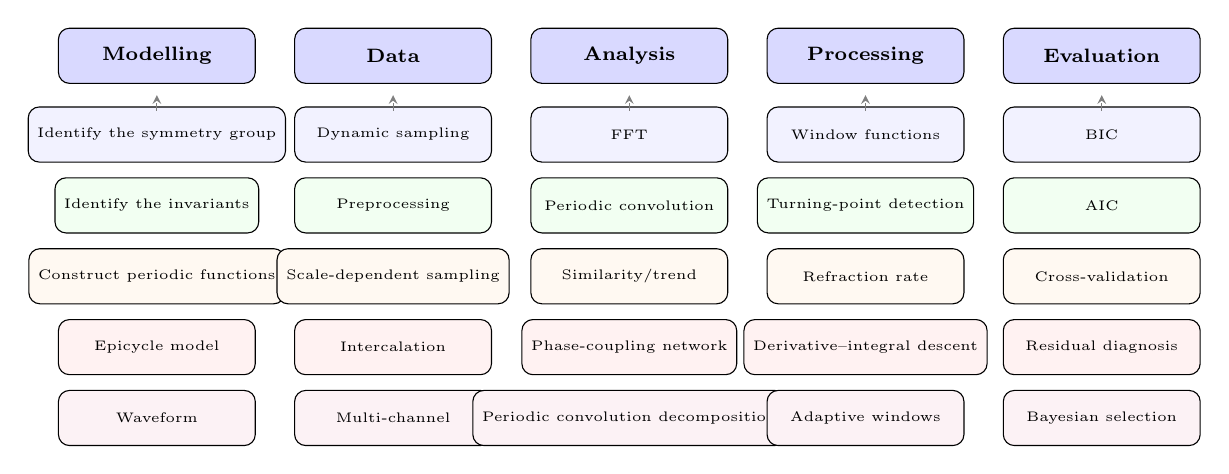
\begin{tikzpicture}[>=stealth,
        story/.style={draw, rounded corners, minimum width=2.5cm, minimum height=0.7cm, align=center, font=\tiny},
        header/.style={draw, rounded corners, fill=blue!15, minimum width=2.5cm, minimum height=0.7cm, align=center, font=\scriptsize\bfseries}]
        
        \node[header] (h1) at (0,4) {Modelling};
        \node[header] (h2) at (3,4) {Data};
        \node[header] (h3) at (6,4) {Analysis};
        \node[header] (h4) at (9,4) {Processing};
        \node[header] (h5) at (12,4) {Evaluation};
        
        \node[story, fill=blue!5] (s11) at (0,3.0) {Identify the symmetry group};
        \node[story, fill=blue!5] (s12) at (3,3.0) {Dynamic sampling};
        \node[story, fill=blue!5] (s13) at (6,3.0) {FFT};
        \node[story, fill=blue!5] (s14) at (9,3.0) {Window functions};
        \node[story, fill=blue!5] (s15) at (12,3.0) {BIC};
        
        \node[story, fill=green!5] (s21) at (0,2.1) {Identify the invariants};
        \node[story, fill=green!5] (s22) at (3,2.1) {Preprocessing};
        \node[story, fill=green!5] (s23) at (6,2.1) {Periodic convolution};
        \node[story, fill=green!5] (s24) at (9,2.1) {Turning-point detection};
        \node[story, fill=green!5] (s25) at (12,2.1) {AIC};
        
        \node[story, fill=orange!5] (s31) at (0,1.2) {Construct periodic functions};
        \node[story, fill=orange!5] (s32) at (3,1.2) {Scale-dependent sampling};
        \node[story, fill=orange!5] (s33) at (6,1.2) {Similarity/trend};
        \node[story, fill=orange!5] (s34) at (9,1.2) {Refraction rate};
        \node[story, fill=orange!5] (s35) at (12,1.2) {Cross-validation};
        
        \node[story, fill=red!5] (s41) at (0,0.3) {Epicycle model};
        \node[story, fill=red!5] (s42) at (3,0.3) {Intercalation};
        \node[story, fill=red!5] (s43) at (6,0.3) {Phase-coupling network};
        \node[story, fill=red!5] (s44) at (9,0.3) {Derivative--integral descent};
        \node[story, fill=red!5] (s45) at (12,0.3) {Residual diagnosis};
        
        \node[story, fill=purple!5] (s51) at (0,-0.6) {Waveform};
        \node[story, fill=purple!5] (s52) at (3,-0.6) {Multi-channel};
        \node[story, fill=purple!5] (s53) at (6,-0.6) {Periodic convolution decomposition};
        \node[story, fill=purple!5] (s54) at (9,-0.6) {Adaptive windows};
        \node[story, fill=purple!5] (s55) at (12,-0.6) {Bayesian selection};
        
        \draw[->, gray, dashed] (0,3.3) -- (0,3.5);
        \draw[->, gray, dashed] (3,3.3) -- (3,3.5);
        \draw[->, gray, dashed] (6,3.3) -- (6,3.5);
        \draw[->, gray, dashed] (9,3.3) -- (9,3.5);
        \draw[->, gray, dashed] (12,3.3) -- (12,3.5);
    \end{tikzpicture}
    \caption{User-story map. The horizontal axis gives the five stages of the methodology (modelling, data, analysis, processing, evaluation), and the vertical axis gives the levels of stories from basic capability to integrated capability. The higher the level, the greater the degree of integration covered by the story; stories at the same level can be delivered independently within that stage.}
    \label{fig:user_story_map}
\end{figure}

\newpage

\section{Business process model (BPMN style)}

\begin{figure}[htbp]
    \centering
    \begin{tikzpicture}[>=stealth,
        start/.style={draw, circle, fill=green!40, minimum size=0.6cm},
        end/.style={draw, circle, fill=red!40, minimum size=0.6cm, double},
        task/.style={draw, rounded corners, fill=blue!10, minimum width=2.2cm, minimum height=0.7cm, align=center, font=\tiny},
        gateway/.style={draw, diamond, fill=yellow!30, minimum size=0.7cm, align=center, font=\tiny},
        arrow/.style={->, thick, >=stealth}]
        
        \node[start] (s) at (0,0) {};
        \node[task] (t1) at (2,0) {Receive data};
        \node[task] (t2) at (4.5,0) {Periodicity detection};
        \node[gateway] (g1) at (7,0) {};
        \node[task] (t3) at (9.5,1.2) {Fit epicycles};
        \node[task] (t4) at (9.5,-1.2) {Adjust the window length};
        \node[task] (t5) at (12,0) {Waveform output};
        \node[end] (e) at (14,0) {};
        
        \draw[arrow] (s) -- (t1);
        \draw[arrow] (t1) -- (t2);
        \draw[arrow] (t2) -- (g1);
        \draw[arrow] (g1) -- node[left, font=\tiny, pos=0.5] {significant} (t3);
        \draw[arrow] (g1) -- node[left, font=\tiny, pos=0.5] {not significant} (t4);
        \draw[arrow] (t4) -- (t2);
        \draw[arrow] (t3) -- (t5);
        \draw[arrow] (t5) -- (e);
        
        \node[font=\tiny, above=0.1cm of g1] {Peak significant?};
    \end{tikzpicture}
    \caption{Business process model of modelling and analysis (BPMN style). It starts with receiving data and proceeds through periodicity detection; if the peak is significant, epicycles are fitted and the Waveform is output; if it is not significant, the window length is adjusted and detection is repeated until it becomes significant or a termination condition is reached.}
    \label{fig:bpmn}
\end{figure}

\newpage

\section{Data flow diagram (DFD)}

\begin{figure}[htbp]
    \centering
    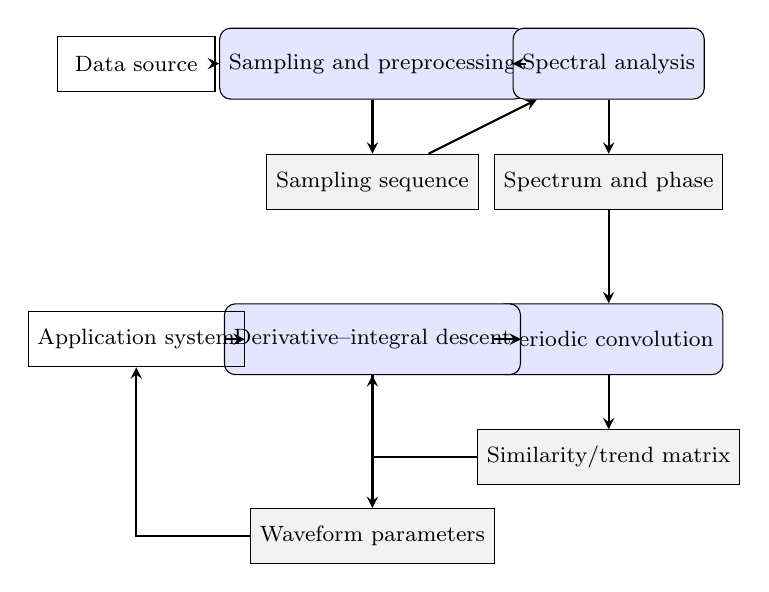
\begin{tikzpicture}[>=stealth,
        proc/.style={draw, rounded corners, fill=blue!10, minimum width=2.4cm, minimum height=0.9cm, align=center, font=\footnotesize},
        store/.style={draw, fill=gray!10, minimum width=2.4cm, minimum height=0.7cm, align=center, font=\footnotesize},
        ext/.style={draw, minimum width=2.0cm, minimum height=0.7cm, align=center, font=\footnotesize},
        arrow/.style={->, thick, >=stealth}]
        
        \node[ext]  (src) at (-4.5,  2.0) {Data source};
        \node[proc] (p1)  at (-1.5,  2.0) {Sampling and preprocessing};
        \node[proc] (p2)  at ( 1.5,  2.0) {Spectral analysis};
        
        \node[store] (ds1) at (-1.5, 0.5) {Sampling sequence};
        \node[store] (ds2) at ( 1.5, 0.5) {Spectrum and phase};
        
        \node[proc] (p3)  at ( 1.5, -1.5) {Periodic convolution};
        \node[proc] (p4)  at (-1.5, -1.5) {Derivative--integral descent};
        \node[ext]  (out) at (-4.5, -1.5) {Application system};
        
        \node[store] (ds3) at ( 1.5, -3.0) {Similarity/trend matrix};
        \node[store] (ds4) at (-1.5, -4.0) {Waveform parameters};
        
        \draw[arrow] (src) -- (p1);
        \draw[arrow] (p1)  -- (p2);
        
        \draw[arrow] (p1)  -- (ds1);
        \draw[arrow] (ds1) -- (p2);
        
        \draw[arrow] (p2)  -- (ds2);
        \draw[arrow] (ds2) -- (p3);
        
        \draw[arrow] (p3)  -- (p4);
        \draw[arrow] (p4)  -- (out);
        
        \draw[arrow] (p3)  -- (ds3);
        
        \draw[arrow] (ds3.west) -| (p4.south);
        
        \draw[arrow] (p4)  -- (ds4);
        
        \draw[arrow] (ds4.west) -| (out.south);
        
    \end{tikzpicture}
    \caption{Data flow diagram (DFD). Data pass from the data source through sampling and preprocessing, spectral analysis, periodic convolution and derivative--integral descent to the application system, with intermediate stores for the sampling sequence, the spectrum and phase, the similarity/trend matrix and the Waveform parameters.}
    \label{fig:dfd}
\end{figure}

\newpage

\section{ER diagram}

\begin{figure}[htbp]
    \centering
    \begin{tikzpicture}[>=stealth,
        ent/.style={draw, fill=blue!10, minimum width=2.8cm, minimum height=0.8cm, align=center, font=\footnotesize\bfseries},
        attr/.style={draw, ellipse, fill=gray!10, minimum width=1.6cm, minimum height=0.6cm, align=center, font=\tiny},
        rel/.style={draw, diamond, fill=yellow!30, minimum size=0.8cm, align=center, font=\tiny},
        link/.style={thick}]
        
        \node[ent] (epi) at (0,3) {Epicycle};
        \node[ent] (wf) at (4,3) {Waveform};
        \node[ent] (ps) at (8,3) {PeriodicSeries};
        \node[ent] (sm) at (0,0) {Sample};
        \node[ent] (sp) at (4,0) {Spectrum};
        \node[ent] (sa) at (8,0) {Sampler};
        
        \node[attr] (a1) at (-2,4.2) {amplitude $A$};
        \node[attr] (a2) at (-2,2.6) {frequency $\omega$};
        \node[attr] (a3) at (0,4.6) {phase $\phi$};
        
        \node[attr] (b1) at (4,4.6) {order $K$};
        \node[attr] (b2) at (6,4.2) {complex-valued function};
        
        \node[attr] (c1) at (8,4.6) {multiple periods};
        \node[attr] (c2) at (10,2.6) {component set};
        
        \node[attr] (d1) at (-2,1) {sample values};
        \node[attr] (d2) at (0,-1) {sampling rate};
        
        \node[attr] (e1) at (4,1) {frequency set};
        \node[attr] (e2) at (4,-1) {amplitude set};
        
        \node[attr] (f1) at (8,1) {transform method};
        
        \node[rel] (r1) at (2,3) {contains};
        \node[rel] (r2) at (6,3) {truncates};
        \node[rel] (r3) at (2,0) {samples};
        \node[rel] (r4) at (6,0) {transforms};
        
        \draw[link] (epi) -- (r1);
        \draw[link] (r1) -- (wf);
        \draw[link] (wf) -- (r2);
        \draw[link] (r2) -- (ps);
        \draw[link] (sm) -- (r3);
        \draw[link] (r3) -- (sp);
        \draw[link] (sp) -- (r4);
        \draw[link] (r4) -- (sa);
        
        \draw[thin] (epi) -- (a1);
        \draw[thin] (epi) -- (a2);
        \draw[thin] (epi) -- (a3);
        \draw[thin] (wf) -- (b1);
        \draw[thin] (wf) -- (b2);
        \draw[thin] (ps) -- (c1);
        \draw[thin] (ps) -- (c2);
        \draw[thin] (sm) -- (d1);
        \draw[thin] (sm) -- (d2);
        \draw[thin] (sp) -- (e1);
        \draw[thin] (sp) -- (e2);
        \draw[thin] (sa) -- (f1);
    \end{tikzpicture}
    \caption{ER diagram. Six entities: Epicycle, Waveform (complex-valued function), PeriodicSeries (periodic series), Sample (sample), Spectrum (spectrum) and Sampler (transformer). The relations are contains, truncates, samples and transforms.}
    \label{fig:er_diagram}
\end{figure}

\newpage

\section{System architecture diagram}

\begin{figure}[htbp]
    \centering
    \begin{tikzpicture}[>=stealth,
        layer/.style={draw, rounded corners, minimum width=12cm, minimum height=1.2cm, align=center, font=\small},
        comp/.style={draw, rounded corners, fill=white, minimum width=2.2cm, minimum height=0.7cm, align=center, font=\tiny},
        arrow/.style={->, thick, >=stealth}]
        
        \node[layer, fill=blue!10] (L1) at (0,4) {\textbf{Application layer (Application)}\\ astronomy, calendars, geography, biology, psychology, economics, politics, algorithms, agents};
        \node[layer, fill=green!10] (L2) at (0,2.5) {\textbf{Modelling and analysis layer (Modelling \& Analysis)}\\ periodic convolution, similarity/trend, derivative--integral descent};
        \node[layer, fill=orange!10] (L3) at (0,1) {\textbf{Data structure layer (Data Structure)}\\ Epicycle, Waveform, PeriodicSeries, Spectrum};
        \node[layer, fill=purple!10] (L4) at (0,-0.5) {\textbf{Primitive operator layer (Primitive Operators)}\\ FFT, Mellin, Laplace, Chirp-Z, wavelet, periodic transform};
        \node[layer, fill=red!10] (L5) at (0,-2) {\textbf{Sampling and observation layer (Sampling \& Observer)}\\ dynamic sampling, intercalation, Nyquist, scale-dependent};
        
        \draw[arrow] (L1.south) -- (L2.north);
        \draw[arrow] (L2.south) -- (L3.north);
        \draw[arrow] (L3.south) -- (L4.north);
        \draw[arrow] (L4.south) -- (L5.north);
        
        \node[font=\tiny, right=0.2cm of L1] {(API)};
        \node[font=\tiny, right=0.2cm of L2] {(Algorithms)};
        \node[font=\tiny, right=0.2cm of L3] {(Classes)};
        \node[font=\tiny, right=0.2cm of L4] {(Transforms)};
        \node[font=\tiny, right=0.2cm of L5] {(Hardware)};
    \end{tikzpicture}
    \caption{System architecture diagram. A five-layer architecture: application layer, modelling and analysis layer, data structure layer, primitive operator layer, and sampling and observation layer. Dependencies between layers run in one direction, from the bottom upwards.}
    \label{fig:architecture}
\end{figure}

\newpage

\section{Program representation of the core classes}

This section maps the core concepts of periodicity mathematics to program representations. The core abstraction is the \textbf{Functor}---every smooth ($C^\infty$) mathematical object that can be differentiated and integrated repeatedly. The class system is divided into three modules: the function class hierarchy, the series class hierarchy, and the integral transform and sampling classes.

\subsection{The Functor class: abstract base class of smooth functions}

\begin{definition}[Functor class]\label{def:functor_class}
\textbf{Functor} is the abstract base class of all smooth functions, that is, of all $C^\infty$ functions. Its core methods are differentiation, integration, limit and evaluation:
\begin{enumerate}[label=(\roman*)]
    \item \texttt{derivative(t)}: returns the derivative of the Functor at $t$---still a Functor.
    \item \texttt{integral(t)}: returns the indefinite integral (primitive function) of the Functor---still a Functor.
    \item \texttt{integral(a, b)}: returns the definite integral (area) of the Functor over the interval $[a,b]$.
    \item \texttt{limit(t)}: returns the limit of the Functor at $t$.
    \item \texttt{evaluate(t)}: returns the value of the Functor at $t$.
\end{enumerate}
The subclasses of Functor include: linear functions, quadratic functions, cubic functions, the sine function, the cosine function, the tangent function, Epicycle, Waveform, Convolution and Series.
\end{definition}

\begin{property}[Closure property of the Functor class]\label{prop:functor_closure}
The Functor class is closed under the following operations:
\begin{enumerate}[label=(\roman*)]
    \item \textbf{Differentiation}: the derivative of a Functor is still a Functor.
    \item \textbf{Integration}: the primitive function of a Functor is still a Functor.
    \item \textbf{Linear combination}: a linear combination of two Functors is still a Functor.
    \item \textbf{Composition}: the composition of two Functors is still a Functor.
    \item \textbf{Convolution}: the convolution of two Functors is still a Functor.
\end{enumerate}
\end{property}

\begin{proof}
(i)(ii) By the fundamental theorem of calculus, the derivative and the primitive function of a $C^\infty$ function are still $C^\infty$ functions.
(iii) The derivative of a linear combination equals the linear combination of the derivatives, so it is still a Functor.
(iv) By the chain rule, the derivative of a composite function exists and can be computed.
(v) By the differentiation property of convolution $(f * g)' = f' * g = f * g'$, the convolution is still a $C^\infty$ function.
\end{proof}

\subsection{Function class hierarchy}

\begin{definition}[Basic function subclasses]\label{def:basic_function_subclasses}
The basic subclasses of Functor include:
\begin{enumerate}[label=(\roman*)]
    \item \textbf{LinearFunction}: $f(t) = at + b$, whose derivative is the constant $a$ and whose primitive function is $\frac{a}{2}t^2 + bt + C$.
    \item \textbf{QuadraticFunction}: $f(t) = at^2 + bt + c$, whose derivative is $2at + b$.
    \item \textbf{CubicFunction}: $f(t) = at^3 + bt^2 + ct + d$.
    \item \textbf{SineFunction}: $f(t) = A\sin(\omega t + \phi)$, whose derivative is $A\omega\cos(\omega t + \phi)$.
    \item \textbf{CosineFunction}: $f(t) = A\cos(\omega t + \phi)$, whose derivative is $-A\omega\sin(\omega t + \phi)$.
    \item \textbf{TangentFunction}: $f(t) = A\tan(\omega t + \phi)$, whose derivative is $A\omega\sec^2(\omega t + \phi)$.
\end{enumerate}
\end{definition}

\begin{proposition}[Derivative closure of basic functions]\label{prop:basic_function_derivative_closure}
The closure relations of the basic function subclasses under differentiation are:
\begin{enumerate}[label=(\roman*)]
    \item $\frac{d}{dt}\operatorname{Sine}(\omega t) = \omega \cdot \operatorname{Cosine}(\omega t)$.
    \item $\frac{d}{dt}\operatorname{Cosine}(\omega t) = -\omega \cdot \operatorname{Sine}(\omega t)$.
    \item $\frac{d}{dt}\operatorname{Tangent}(\omega t) = \omega \cdot \operatorname{Secant}^2(\omega t)$.
\end{enumerate}
The sine and the cosine are interconverted under differentiation, forming a closed orbit of period $2$.
\end{proposition}

\begin{proof}
This follows by direct verification from the basic derivative formulae. Differentiating the sine function gives the cosine function, and differentiating the cosine function gives minus the sine function; after two differentiations one returns to the original function (up to a sign), forming a $C_2$ involution structure (\cref{def:group_action}).
\end{proof}

\begin{definition}[Epicycle class]\label{def:epicycle_class}
The \textbf{Epicycle} class inherits from Functor and represents a single epicycle:
\[
\gamma(t) = A e^{i(\omega t + \phi)}.
\]
Its fields are the amplitude $A$, the angular frequency $\omega$ and the initial phase $\phi$. The Epicycle is the most basic geometric unit in periodicity mathematics and is also a constituent element of the Waveform (its mathematical object being that of \cref{def:epicycle}).
\end{definition}

\begin{property}[Method semantics of the Epicycle class]\label{prop:epicycle_class_methods}
\begin{enumerate}[label=(\roman*)]
    \item \texttt{derivative(t)}: returns $\omega A e^{i(\omega t + \phi + \pi/2)}$---the amplitude is multiplied by $\omega$ and the phase is increased by $\pi/2$.
    \item \texttt{integral(t)}: returns $\frac{A}{\omega} e^{i(\omega t + \phi - \pi/2)}$---the amplitude is divided by $\omega$ and the phase is decreased by $\pi/2$.
    \item \texttt{integral(a, b)}: returns $\frac{A}{i\omega}(e^{i(\omega b + \phi)} - e^{i(\omega a + \phi)})$.
    \item \texttt{evaluate(t)}: returns $A e^{i(\omega t + \phi)}$.
    \item \texttt{convolute(Epicycle, Delay)}: returns the periodic convolution of two Epicycles under a given time delay (\cref{def:periodic_convolution}).
    \item \texttt{similarity(Epicycle)}: returns the similarity of two Epicycles (\cref{def:similarity_essence}).
    \item \texttt{tendency(Epicycle)}: returns the trend of two Epicycles (\cref{def:tendency}).
\end{enumerate}
\end{property}

\begin{proof}
Derivative: $\frac{d}{dt}Ae^{i(\omega t + \phi)} = i\omega A e^{i(\omega t + \phi)} = \omega A e^{i(\omega t + \phi + \pi/2)}$.
Integral: $\int Ae^{i(\omega t + \phi)}dt = \frac{A}{i\omega}e^{i(\omega t + \phi)} = \frac{A}{\omega}e^{i(\omega t + \phi - \pi/2)}$.
The definite integral follows directly from the fundamental theorem of calculus. The convolution, similarity and trend are computed componentwise from the definitions of \cref{def:periodic_convolution,def:similarity_essence,def:tendency}.
\end{proof}

\begin{definition}[Waveform class]\label{def:waveform_class}
The \textbf{Waveform} class inherits from Functor and represents a complex-valued function composed of several Epicycles (its mathematical object being that of \cref{def:waveform_definition}):
\[
\mathcal{W}(t) = \sum_{k=1}^{K} A_k e^{i(\omega_k t + \phi_k)}.
\]
Internally it uses a double-ended queue to store Epicycle objects. A Waveform is both a Functor (differentiable and integrable) and a container of Epicycles (epicycles may be added and removed).
\end{definition}

\begin{property}[Method semantics of the Waveform class]\label{prop:waveform_class_methods}
\begin{enumerate}[label=(\roman*)]
    \item Queue operations: \texttt{pushFront}, \texttt{removeFront}, \texttt{pushBack}, \texttt{removeBack}, \texttt{removeAt}---these support the dynamic addition and removal of epicycles.
    \item \texttt{front()} / \texttt{back()}: returns the first or the last Epicycle.
    \item Functor interface: \texttt{derivative(t)}, \texttt{integral(t)}, \texttt{integral(a,b)}, \texttt{limit(t)}, \texttt{evaluate(t)}---these act componentwise on each Epicycle.
    \item \texttt{convolute(Waveform, Delay)}: returns the periodic convolution of two Waveforms.
    \item \texttt{similarity(Waveform)}: returns the similarity matrix of two Waveforms.
    \item \texttt{tendency(Waveform)}: returns the trend matrix of two Waveforms.
\end{enumerate}
\end{property}

\begin{proof}
The Functor methods of the Waveform are the componentwise extension of the corresponding methods of the Epicycle. Since the Waveform is a finite sum of Epicycles, the linear operations (differentiation, integration) may be carried out componentwise. The convolution, similarity and trend are computed componentwise from the definitions of \cref{def:periodic_convolution,def:similarity_essence,def:tendency}.
\end{proof}

\begin{definition}[Convolution class]\label{def:convolution_class}
The \textbf{Convolution} class inherits from Functor and represents the convolution of two Functors:
\[
(f * g)(t) = \int_{-\infty}^{\infty} f(\tau) g(t - \tau) d\tau.
\]
A Convolution is itself a Functor---differentiable and integrable. Its mathematical object is that of \cref{def:convolution}.
\end{definition}

\begin{property}[Differentiation property of the Convolution class]\label{prop:convolution_class_derivative}
\[
(f * g)' = f' * g = f * g'.
\]
The derivative of a convolution equals the convolution of the derivative of either factor with the other factor.
\end{property}

\begin{proof}
This follows directly from \cref{prop:convolution_properties}(v). This is the key property of convolution as a Functor---it guarantees the closure of convolution within the Functor class.
\end{proof}

\newpage

\begin{figure}[htbp]
    \centering
    \begin{tikzpicture}[>=stealth,
        classbox/.style={draw, rectangle, minimum width=2.8cm, align=left, font=\scriptsize, inner sep=4pt},
        inherit/.style={->, thick, >=open triangle 60, dashed}]
        
        \node[classbox, fill=orange!10, minimum height=1.2cm] (linear) at (-4.0,5.0) {\textbf{LinearFunction}\\ \texttt{+ a, b}};
        \node[classbox, fill=orange!10, minimum height=1.2cm] (quadratic) at (0,5.0) {\textbf{QuadraticFunction}\\ \texttt{+ a, b, c}};
        \node[classbox, fill=orange!10, minimum height=1.2cm] (cubic) at (4.0,5.0) {\textbf{CubicFunction}\\ \texttt{+ a, b, c, d}};
        
        \node[classbox, fill=orange!10, minimum height=1.2cm] (exponential) at (-6,1.5) {\textbf{ExponentialFunction}\\ \texttt{+ base}};
        \node[classbox, fill=orange!10, minimum height=1.2cm] (logarithmic) at (-6,0) {\textbf{LogarithmicFunction}\\ \texttt{+ base}};
        \node[classbox, fill=orange!10, minimum height=1.2cm] (power) at (-6,-1.5) {\textbf{PowerFunction}\\ \texttt{+ exponent}};
        
        \node[classbox, fill=gray!10, minimum height=2.8cm] (functor) at (0,0) {
            \textbf{Functor}\\[2pt]
            \texttt{+ derivative(t)}\\
            \texttt{+ integral(t)}\\
            \texttt{+ integral(a, b)}\\
            \texttt{+ limit(t)}\\
            \texttt{+ evaluate(t)}
        };
        
        \node[classbox, fill=orange!10, minimum height=1.2cm] (sine) at (6,1.5) {\textbf{SineFunction}\\ \texttt{+ A, omega, phi}};
        \node[classbox, fill=orange!10, minimum height=1.2cm] (cosine) at (6,0) {\textbf{CosineFunction}\\ \texttt{+ A, omega, phi}};
        \node[classbox, fill=orange!10, minimum height=1.2cm] (tangent) at (6,-1.5) {\textbf{TangentFunction}\\ \texttt{+ A, omega, phi}};
        
        \node[classbox, fill=blue!10, minimum height=1.8cm] (epicycle) at (-4.0,-4.5) {
            \textbf{Epicycle}\\[2pt]
            \texttt{+ amplitude}\\
            \texttt{+ omega}\\
            \texttt{+ phase}
        };
        
        \node[classbox, fill=green!10, minimum height=1.8cm] (waveform) at (0,-4.5) {
            \textbf{Waveform}\\[2pt]
            \texttt{+ epicicles}\\
            \texttt{+ push / remove}\\
            \texttt{+ convolute}\\
            \texttt{+ similarity}\\
            \texttt{+ tendency}
        };
        
        \node[classbox, fill=red!10, minimum height=1.8cm] (convolution) at (4.0,-4.5) {
            \textbf{Convolution}\\[2pt]
            \texttt{+ f : Functor}\\
            \texttt{+ g : Functor}
        };
        
        \draw[inherit] (linear.south) -- (functor.north);
        \draw[inherit] (quadratic.south) -- (functor.north);
        \draw[inherit] (cubic.south) -- (functor.north);
        \draw[inherit] (exponential.east) -- (functor.west);
        \draw[inherit] (logarithmic.east) -- (functor.west);
        \draw[inherit] (power.east) -- (functor.west);
        \draw[inherit] (sine.west) -- (functor.east);
        \draw[inherit] (cosine.west) -- (functor.east);
        \draw[inherit] (tangent.west) -- (functor.east);
        \draw[inherit] (epicycle.north) -- (functor.south);
        \draw[inherit] (waveform.north) -- (functor.south);
        \draw[inherit] (convolution.north) -- (functor.south);
        \draw[->, thick, >=stealth] (waveform.west) -- node[above, font=\tiny] {contains} (epicycle.east);
    \end{tikzpicture}
    \caption{Function class hierarchy (UML class diagram). Functor is the abstract base class of all differentiable functions. Above are the algebraic functions (linear, quadratic, cubic), to the left are the transcendental functions (exponential, logarithmic, power), to the right are the trigonometric functions (sine, cosine, tangent), and below are the core classes of periodicity mathematics (Epicycle, Waveform, Convolution). The Waveform contains a set of Epicycles.}
    \label{fig:uml_functor_hierarchy}
\end{figure}

\newpage

\subsection{Series class hierarchy}

\begin{definition}[Series class]\label{def:series_class}
The \textbf{Series} class inherits from Functor and represents a series of functions:
\[
S(t) = \sum_{k=0}^{\infty} u_k(t).
\]
Its fields are the sequence of terms \texttt{terms: Deque<Functor>} and the centre of expansion \texttt{center: Number}. The subclasses of Series include the Taylor series, the Fourier series, the Laurent series and the periodic series.
\end{definition}

\begin{property}[Method semantics of the Series class]\label{prop:series_class_methods}
\begin{enumerate}[label=(\roman*)]
    \item \texttt{evaluate(t)}: returns the partial sum of the series at $t$ (taking the first $n$ terms).
    \item \texttt{truncate(n)}: returns the series truncated to the first $n$ terms.
    \item \texttt{derivative(t)}: differentiates term by term and returns a new Series.
    \item \texttt{integral(t)}: integrates term by term and returns a new Series.
    \item \texttt{convergeRadius()}: returns the radius of convergence of the series (for Taylor/Laurent series; for Fourier/periodic series it returns $\infty$ or is defined in terms of the period length).
\end{enumerate}
\end{property}

\begin{proof}
The term-by-term differentiation and integration of the series are guaranteed by uniform convergence (\cref{thm:uniform_termwise_integration,thm:uniform_termwise_differentiation}). The radius of convergence is computed by the Cauchy--Hadamard formula (\cref{thm:cauchy_hadamard}).
\end{proof}

\begin{definition}[Program representation of the Taylor series]\label{def:taylor_series_class}
The mathematical object represented by this class is the Taylor series defined in \cref{def:taylor_series}; here only its program representation (class name and inheritance relation) is given, and the mathematical object is not redefined. \textbf{TaylorSeries} inherits from Series and represents the Taylor expansion of a function at $t_0$:
\[
f(t) = \sum_{k=0}^{\infty} \frac{f^{(k)}(t_0)}{k!}(t - t_0)^k.
\]
\end{definition}

\begin{definition}[Program representation of the Fourier series]\label{def:fourier_series_class}
The mathematical object represented by this class is the Fourier series defined in \cref{def:fourier_series_foundations}; here only its program representation (class name and inheritance relation) is given, and the mathematical object is not redefined. \textbf{FourierSeries} inherits from Series and represents the Fourier expansion of a periodic function:
\[
f(t) = \sum_{n=-\infty}^{\infty} c_n e^{i 2\pi n t / T}.
\]
\end{definition}

\begin{definition}[Program representation of the Laurent series]\label{def:laurent_series_class}
The mathematical object represented by this class is the Laurent series defined in \cref{def:laurent_series}; here only its program representation (class name and inheritance relation) is given, and the mathematical object is not redefined. \textbf{LaurentSeries} inherits from Series and represents the Laurent expansion of an analytic function:
\[
f(z) = \sum_{n=-\infty}^{\infty} a_n (z - z_0)^n.
\]
\end{definition}

\begin{definition}[Program representation of the periodic series]\label{def:periodic_series_class}
\textbf{PeriodicSeries} inherits from Series and represents the periodic series expansion of a multi-periodic function (its mathematical object being that of \cref{def:periodic_series}):
\[
f(t) = \sum_{p \in P} \sum_{n \in \mathbb{Z}} A_{p,n} e^{i(\omega_{p,n} t + \phi_{p,n})}.
\]
\end{definition}

\begin{proposition}[Relation between Series and Waveform]\label{prop:series_waveform_relation}
A finite truncation of a PeriodicSeries is equivalent to a Waveform. Specifically, after a PeriodicSeries has been truncated to finitely many terms, every element of its sequence of terms is an Epicycle, so it can be converted into a Waveform.
\end{proposition}

\begin{proof}
Each term $A_{p,n} e^{i(\omega_{p,n} t + \phi_{p,n})}$ of the PeriodicSeries is an Epicycle (\cref{def:epicycle_class}). After truncation to finitely many terms, the sequence of terms constitutes a set of Epicycles, that is, a Waveform (\cref{def:waveform_class}). The conversion is carried out by the \texttt{toWaveform()} method.
\end{proof}

\newpage

\begin{figure}[htbp]
    \centering
    \begin{tikzpicture}[>=stealth,
        classbox/.style={draw, rectangle, minimum width=3.2cm, align=left, font=\scriptsize, inner sep=4pt},
        inherit/.style={->, thick, >=open triangle 60, dashed}]
        
        \node[classbox, fill=cyan!10, minimum height=3cm] (series) at (0,2) {
            \textbf{Series}\\[2pt]
            \texttt{+ terms : Deque<Functor>}\\
            \texttt{+ center : Number}\\[2pt]
            \texttt{+ truncate(n)}\\
            \texttt{+ convergeRadius()}
        };
        
        \node[classbox, fill=cyan!20, minimum height=1.5cm] (taylor) at (-7,-1) {\textbf{TaylorSeries}\\ \texttt{+ f : Functor}\\ \texttt{+ t0 : Number}};
        \node[classbox, fill=cyan!20, minimum height=1.5cm] (fourier) at (-3,-1) {\textbf{FourierSeries}\\ \texttt{+ period : Number}\\ \texttt{+ coeffs : Deque}};
        \node[classbox, fill=cyan!20, minimum height=1.5cm] (laurent) at (1,-1) {\textbf{LaurentSeries}\\ \texttt{+ z0 : Number}\\ \texttt{+ annulus : Range}};
        \node[classbox, fill=cyan!20, minimum height=1.5cm] (periodic) at (5,-1) {\textbf{PeriodicSeries}\\ \texttt{+ periods : Deque}\\ \texttt{+ components}};
        
        \draw[inherit] (taylor.north) -- (series.south);
        \draw[inherit] (fourier.north) -- (series.south);
        \draw[inherit] (laurent.north) -- (series.south);
        \draw[inherit] (periodic.north) -- (series.south);
    \end{tikzpicture}
    \caption{Series class hierarchy (UML class diagram). Series inherits from Functor, and its subclasses include the Taylor series, the Fourier series, the Laurent series and the periodic series.}
    \label{fig:uml_series_hierarchy}
\end{figure}

\newpage

\subsection{Integral transform and sampling classes}

\begin{definition}[Spectrum class]\label{def:spectrum_class}
The \textbf{Spectrum} class represents a spectrum---a double-ended queue composed of several Spectral components. The \texttt{toWaveform()} method converts a spectrum into a Waveform.
\end{definition}

\begin{definition}[Spectral class]\label{def:spectral_class}
The \textbf{Spectral} class represents a single spectral component, with the fields frequency, amplitude and phase. The \texttt{toEpicycle()} method converts a spectral component into an epicycle.
\end{definition}

\begin{definition}[Sample class]\label{def:sample_class}
The \textbf{Sample} class represents sampled data, with the fields sequence of sample values, sampling rate and duration. The \texttt{toWaveform()} method converts sampled data into a Waveform.
\end{definition}

\begin{definition}[Sampler class]\label{def:sampler_class}
\emergencystretch=6em
The \textbf{Sampler} class is a static utility class operating on Waveforms and Spectra. Its methods include:
\begin{enumerate}[label=(\roman*)]
\rightskip=0pt plus1fil\relax
    \item Sampling and resampling: \texttt{sample(Waveform)}, \texttt{resample(Sample)}.
    \item The Fourier transform family: \texttt{fourierTransform}, \texttt{radix2}, \texttt{radix3}, \texttt{radix5}, \texttt{radix7}, \texttt{blueStein}, \texttt{fastFourierC}.
    \item Integral transforms: \texttt{meilinTransform}, \texttt{laplacianTransform}, \texttt{chirpZTransform}, \texttt{waveletTransform}.
\end{enumerate}
\end{definition}

\begin{remark}[Correspondence between the methods of the Sampler class and mathematical transforms]\label{prop:sampler_methods}
Each method of the Sampler class corresponds to a concrete mathematical transform, whose definition may be found in the standard literature on harmonic analysis:
\begin{itemize}
    \item \texttt{fourierTransform} corresponds to the Fourier transform (\cref{def:fourier_transform});
    \item \texttt{radix2/3/5/7} corresponds to the fast Fourier transform (\cref{thm:radix2_fft,thm:radix_p_fft});
    \item \texttt{blueStein} corresponds to the Bluestein algorithm (\cref{prop:bluestein});
    \item \texttt{meilinTransform} corresponds to the Mellin transform (\cref{def:mellin});
    \item \texttt{laplacianTransform} corresponds to the Laplace transform (\cref{def:laplace});
    \item \texttt{chirpZTransform} corresponds to the Chirp-Z transform;
    \item \texttt{waveletTransform} corresponds to the wavelet transform (\cref{def:wavelet_transform});
    \item \texttt{periodicTransform} corresponds to the periodic transform (\cref{def:periodic_transform}).
\end{itemize}
\textbf{This remark is an interface convention and constitutes no new mathematical proposition}. It states that each method of the Sampler class is a program wrapper around an existing mathematical transform; the concrete definitions and convergence conditions are given in the corresponding chapters.
\end{remark}

\newpage

\begin{figure}[htbp]
    \centering
    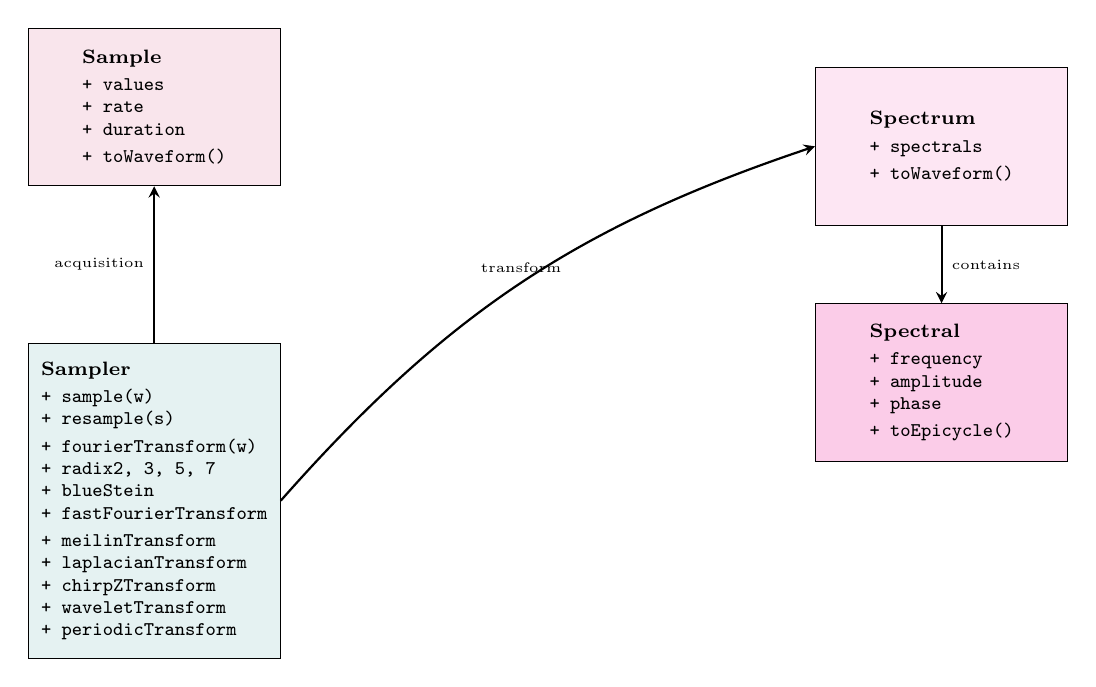
\begin{tikzpicture}[>=stealth,
        classbox/.style={draw, rectangle, minimum width=3.2cm, align=left, font=\scriptsize, inner sep=4pt},
        arrow/.style={->, thick, >=stealth}]
        
        \node[classbox, fill=magenta!10, minimum height=2cm] (spectrum) at (4,2) {\textbf{Spectrum}\\[2pt] \texttt{+ spectrals}\\[2pt] \texttt{+ toWaveform()}};
        \node[classbox, fill=magenta!20, minimum height=2cm] (spectral) at (4,-1) {\textbf{Spectral}\\[2pt] \texttt{+ frequency}\\ \texttt{+ amplitude}\\ \texttt{+ phase}\\[2pt] \texttt{+ toEpicycle()}};
        \node[classbox, fill=purple!10, minimum height=2cm] (sample) at (-6,2.5) {\textbf{Sample}\\[2pt] \texttt{+ values}\\ \texttt{+ rate}\\ \texttt{+ duration}\\[2pt] \texttt{+ toWaveform()}};
        \node[classbox, fill=teal!10, minimum height=4cm] (sampler) at (-6,-2.5) {
            \textbf{Sampler}\\[2pt]
            \texttt{+ sample(w)}\\
            \texttt{+ resample(s)}\\[2pt]
            \texttt{+ fourierTransform(w)}\\
            \texttt{+ radix2, 3, 5, 7}\\
            \texttt{+ blueStein}\\
            \texttt{+ fastFourierTransform}\\[2pt]
            \texttt{+ meilinTransform}\\
            \texttt{+ laplacianTransform}\\
            \texttt{+ chirpZTransform}\\
            \texttt{+ waveletTransform}\\
            \texttt{+ periodicTransform}
        };
        
        \draw[arrow] (spectrum.south) -- node[right, font=\tiny] {contains} (spectral.north);
        \draw[arrow] (sampler.north) -- node[left, font=\tiny, pos=0.5] {acquisition} (sample.south);
        \draw[arrow] (sampler.east) to[bend left=15] node[above, font=\tiny, pos=0.5] {transform} (spectrum.west);
    \end{tikzpicture}
    \caption{Integral transform and sampling classes (UML class diagram). The Sampler is responsible for sampling and the various integral transforms, Sample is the result of sampling, and Spectrum is the spectrum (composed of several Spectral components).}
    \label{fig:uml_transform_sampling}
\end{figure}

\newpage

\subsection{Overall module relation diagram}

\begin{figure}[htbp]
    \centering
    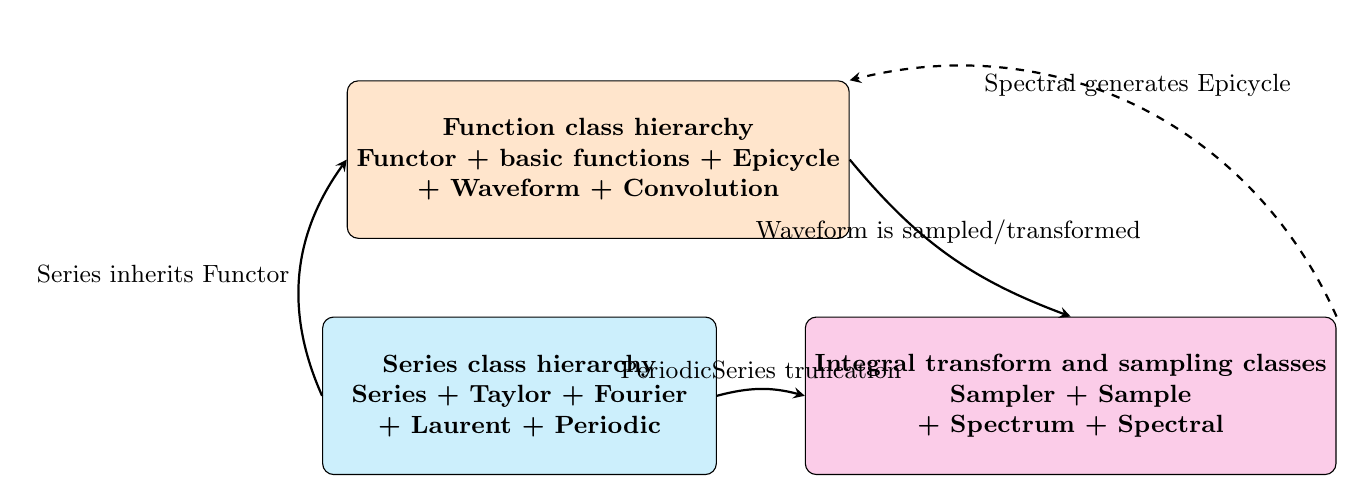
\begin{tikzpicture}[>=stealth,
        module/.style={draw, rounded corners, minimum width=5cm, minimum height=2cm, align=center, font=\small\bfseries},
        arrow/.style={->, thick, >=stealth}]
        
        \node[module, fill=orange!20] (functor_mod) at (0,3) {Function class hierarchy\\Functor + basic functions + Epicycle\\+ Waveform + Convolution};
        \node[module, fill=cyan!20] (series_mod) at (-1,0) {Series class hierarchy\\Series + Taylor + Fourier\\+ Laurent + Periodic};
        \node[module, fill=magenta!20] (transform_mod) at (6,0) {Integral transform and sampling classes\\Sampler + Sample\\+ Spectrum + Spectral};
        
        \draw[arrow] (series_mod.west) to[bend left=30] node[left, font=\small] {Series inherits Functor} (functor_mod.west);
        \draw[arrow] (series_mod.east) to[bend left=15] node[above, font=\small] {PeriodicSeries truncation} (transform_mod.west);
        \draw[arrow] (functor_mod.east) to[bend right=15] node[above, font=\small] {Waveform is sampled/transformed} (transform_mod.north);
        \draw[arrow, dashed, thick] (transform_mod.north east) to[bend right=40] node[above, font=\small] {Spectral generates Epicycle} (functor_mod.north east);
    \end{tikzpicture}
    \caption{Overall module relation diagram. The three modules are interconnected by the relations of inheritance, truncation, sampling/transformation and generation.}
    \label{fig:uml_module_relations}
\end{figure}

\newpage

\section{UML object diagram: a concrete instance}

\begin{figure}[htbp]
    \centering
    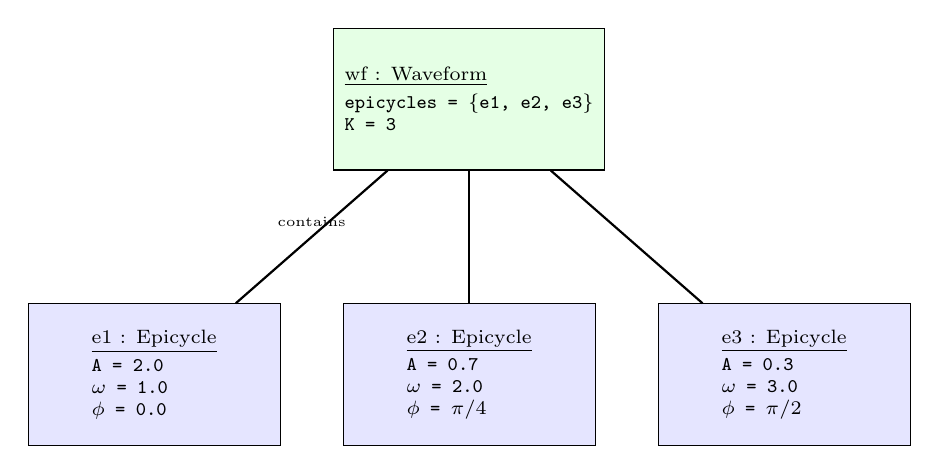
\begin{tikzpicture}[>=stealth,
        obj/.style={draw, rectangle, fill=blue!10, minimum width=3.2cm, minimum height=1.8cm, align=left, font=\scriptsize, inner sep=4pt},
        link/.style={thick}]
        
        \node[obj, fill=green!10] (wf) at (0,2) {
            \underline{wf : Waveform}\\[2pt]
            \texttt{epicycles = \{e1, e2, e3\}}\\
            \texttt{K = 3}
        };
        
        \node[obj] (e1) at (-4,-1.5) {
            \underline{e1 : Epicycle}\\[2pt]
            \texttt{A = 2.0}\\
            \texttt{$\omega$ = 1.0}\\
            \texttt{$\phi$ = 0.0}
        };
        
        \node[obj] (e2) at (0,-1.5) {
            \underline{e2 : Epicycle}\\[2pt]
            \texttt{A = 0.7}\\
            \texttt{$\omega$ = 2.0}\\
            \texttt{$\phi$ = $\pi/4$}
        };
        
        \node[obj] (e3) at (4,-1.5) {
            \underline{e3 : Epicycle}\\[2pt]
            \texttt{A = 0.3}\\
            \texttt{$\omega$ = 3.0}\\
            \texttt{$\phi$ = $\pi/2$}
        };
        
        \draw[link] (wf) -- node[above, font=\tiny] {contains} (e1);
        \draw[link] (wf) -- (e2);
        \draw[link] (wf) -- (e3);
    \end{tikzpicture}
    \caption{UML object diagram. A Waveform instance \texttt{wf} containing three Epicycle instances \texttt{e1}, \texttt{e2} and \texttt{e3}. Each object displays its run-time field values, and this is a concrete instance of the class diagram (\cref{fig:uml_functor_hierarchy}).}
    \label{fig:uml_object_diagram}
\end{figure}

\newpage

\section{UML sequence diagram: from data to Waveform}

\begin{figure}[htbp]
    \centering
    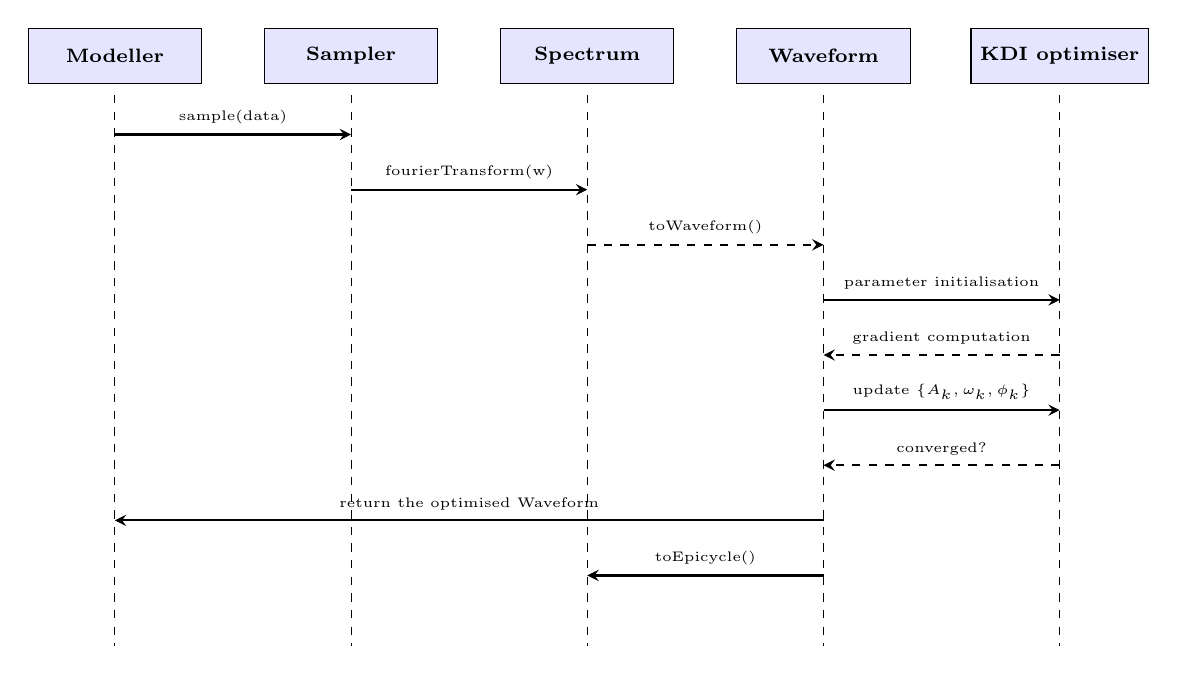
\begin{tikzpicture}[>=stealth,
        lifeline/.style={draw, fill=blue!10, minimum width=2.2cm, minimum height=0.7cm, align=center, font=\scriptsize\bfseries},
        act/.style={draw, fill=white, minimum width=2.2cm, minimum height=0.5cm, align=center, font=\tiny},
        msg/.style={->, thick, >=stealth}]
        
        \node[lifeline] (user) at (0,0) {Modeller};
        \node[lifeline] (samp) at (3,0) {Sampler};
        \node[lifeline] (spec) at (6,0) {Spectrum};
        \node[lifeline] (wave) at (9,0) {Waveform};
        \node[lifeline] (kdi) at (12,0) {KDI optimiser};
        
        \foreach \x in {0,3,6,9,12} {
            \draw[dashed] (\x,-0.5) -- (\x,-7.5);
        }
        
        \draw[msg] (0,-1) -- node[above, font=\tiny] {sample(data)} (3,-1);
        \draw[msg] (3,-1.7) -- node[above, font=\tiny] {fourierTransform(w)} (6,-1.7);
        \draw[msg, dashed] (6,-2.4) -- node[above, font=\tiny] {toWaveform()} (9,-2.4);
        \draw[msg] (9,-3.1) -- node[above, font=\tiny] {parameter initialisation} (12,-3.1);
        \draw[msg, dashed] (12,-3.8) -- node[above, font=\tiny] {gradient computation} (9,-3.8);
        \draw[msg] (9,-4.5) -- node[above, font=\tiny] {update $\{A_k,\omega_k,\phi_k\}$} (12,-4.5);
        \draw[msg, dashed] (12,-5.2) -- node[above, font=\tiny] {converged?} (9,-5.2);
        \draw[msg] (9,-5.9) -- node[above, font=\tiny] {return the optimised Waveform} (0,-5.9);
        \draw[msg] (9,-6.6) -- node[above, font=\tiny] {toEpicycle()} (6,-6.6);
    \end{tikzpicture}
    \caption{UML sequence diagram. The modeller initiates a sampling request, the Sampler completes the spectral analysis, the Spectrum is converted into a Waveform, the KDI optimiser iteratively updates the parameters until convergence, and finally the optimised Waveform and its Epicycle components are returned.}
    \label{fig:uml_sequence}
\end{figure}

\newpage

\section{Modelling: from real-world problems to periodic mathematical models}

\begin{definition}[Steps of modelling]\label{def:modelling_steps}
Modelling is the systematic procedure that abstracts a real-world problem into a periodic mathematical model:
\begin{enumerate}[label=(\roman*)]
    \item \textbf{Identify the transformation group}: determine the basic transformations present in the system and their symmetry group.
    \item \textbf{Identify the invariants}: determine the invariants of the system under the action of the transformation group.
    \item \textbf{Construct periodic functions}: express the state variables of the system as periodic functions (subclasses of Functor).
    \item \textbf{Construct the epicycle model}: expand the periodic functions into a nested epicycle system (Waveform).
    \item \textbf{Determine the coupling relations}: determine the periodic-convolution coupling between the subsystems (Convolution).
\end{enumerate}
\end{definition}

\begin{remark}[Completeness of the modelling steps (empirical observation / research programme)]\label{prop:modelling_completeness}
The five steps above cover the necessary stages from a real-world system to a periodic mathematical model; this is an \textbf{empirical observation / research programme}, not a proved theorem: `completeness' is not defined relative to any class of models, and no verifiable criterion is supplied (for example, `given the state--observation map of any real-world system, the composite of the five steps yields an isomorphic Waveform representation'), so it is used here only as a methodological convention.
The basis of each step is as follows: steps (i)(ii) determine the symmetry and the invariants of the system, where \textbf{symmetry is a necessary condition for periodic structure} (period $\Rightarrow$ symmetry, see \cref{cor:true_logic}), whilst the identification of invariants is a tool for describing the stratification between orbits and is \textbf{not a precondition for the existence of periods} (there exist uniformly periodic systems all of whose conserved quantities are constant); step (iii) expresses the system state as a periodic function (Functor), which is the core of mathematical modelling, see \cref{def:periodic_series}; step (iv) expands the periodic function into epicycles (Waveform), which is the key to the periodic series representation; step (v) determines the periodic-convolution coupling between subsystems, see \cref{def:convolution}.
\end{remark}

\section{Data: acquisition and preprocessing}

\begin{definition}[Periodic mathematical framework for data acquisition]\label{def:data_acquisition}
Data acquisition uses the \textbf{scale-dependent sampling} model: the sampling rate $R(r,\sigma)$ and the number of sampling points $N(r,\sigma)$ are determined by the observer scale $\sigma$ and the observation distance $r$; their definition and monotonicity are given in the `Discrete Sampling and Intercalation of Periodic Signals' chapter, \cref{def:dynamic_sampling}, \cref{prop:sampling_monotonicity}. The sampling theorem (\cref{thm:nyquist_shannon_parallel}) guarantees that, when the sampling rate satisfies the Nyquist condition, a periodic function can be reconstructed uniquely from its sampled values.
\end{definition}

\begin{remark}[Monotonicity of dynamic sampling (citation)]\label{prop:dynamic_sampling_monotonicity}
This proposition is identical with \cref{prop:sampling_monotonicity} of the `Discrete Sampling and Intercalation of Periodic Signals' chapter: for fixed $\sigma>0$, $R$ and $N$ are strictly decreasing in the distance $r$; for fixed $r\ge0$, $R$ and $N$ are strictly increasing in the scale $\sigma$. Both the statement and the proof are to be found there and are not repeated here.
\end{remark}

\section{Analysis: periodic convolution and spectral decomposition}

\begin{definition}[The complete toolchain for analysis]\label{def:analysis_toolchain}
\begin{enumerate}[label=(\roman*)]
    \item \textbf{Classical integral transforms}: the Fourier, wavelet, Mellin, Laplace and Chirp-Z transforms.
    \item \textbf{Similarity transform} ($\alpha=0$): determined by the phase similarity alone (\cref{def:similarity_essence}).
    \item \textbf{Trend transform} ($\alpha=1$): determined jointly by the amplitude and the phase similarity (\cref{def:tendency}).
    \item \textbf{Weight kernels}: kernel functions such as the Gaussian, the Mexican hat and the Cauchy kernel (\cref{def:window_function}).
\end{enumerate}
\end{definition}

\begin{proposition}[Hierarchy of the analysis toolchain]\label{prop:analysis_hierarchy}
The four analysis tools form an inclusion relation with respect to their \textbf{range of information retention} (each later one retains all the information of the former and adds a new dimension):
\[
\text{classical transform} \subset \text{trend transform} \subset \text{similarity transform} \subset \text{weight kernel}
\]
\end{proposition}

\begin{proof}
(Level 1 $\to$ level 2) A classical integral transform gives only the spectral coefficients $c_k$ of a single function; the trend transform retains the amplitude and phase interaction $\mathbb{T}_{mn} = A_n B_m e^{i(\phi_n - \psi_m)}$ of two functions, and its diagonal terms degenerate to the classical transform (\cref{prop:periodic_transform_vs_classical}).

(Level 2 $\to$ level 3) The trend transform contains the amplitude product $A_n B_m$; the similarity transform discards the amplitude information and retains only the phase relation $\mathbb{P}_{mn} = e^{i(\phi_n - \psi_m)}$---it is the special case of the trend transform in which the amplitudes take the values $A_n = B_m = 1$.

(Level 3 $\to$ level 4) The similarity transform gives the same phase kernel for every frequency pair $(n,m)$; the weight kernel weights the frequency pairs through a window function $W$, thereby realising a \textbf{non-uniform} kernel strength on the individual frequency pairs---a degree of freedom that the similarity transform does not possess.

Hence the ranges of information retention of the four form a strict inclusion relation.
\end{proof}

\section{Processing: window functions and derivative--integral descent optimisation}

\begin{definition}[Tools for processing]\label{def:processing_tools}
\begin{enumerate}[label=(\roman*)]
    \item \textbf{Window-function smoothing}: multi-scale smoothing using Gaussian kernels, Cauchy kernels and the like (\cref{def:window_function}).
    \item \textbf{Turning-point detection}: using the criterion of directional change of the instantaneous limit angle (\cref{def:ts_turning_point,def:limit_angle}).
    \item \textbf{Refraction-rate computation}: the difference of the sine trends on the two sides of a turning point (\cref{def:ts_refraction}).
    \item \textbf{Derivative--integral descent optimisation}: the kernel-function derivative--integral descent method (\cref{def:kdi_definition}).
\end{enumerate}
\end{definition}

\begin{proposition}[Division of labour among the processing tools]\label{prop:processing_division}
Window-function smoothing is responsible for noise suppression, turning-point detection for the identification of direction reversals, refraction-rate computation for the quantification of reversal strength, and derivative--integral descent optimisation for the fine adjustment of parameters. The four tools work together to complete the whole processing chain from raw data to a refined signal.
\end{proposition}

\begin{proof}
Each tool addresses one particular aspect of signal processing:
\begin{itemize}
    \item Window-function smoothing (\cref{def:window_function}): suppresses high-frequency noise with $|\omega| > 1/\Delta$ by convolution with $P * K_\Delta$ (\cref{ch29_window_spectral});
    \item Turning-point detection (\cref{def:ts_turning_point}): identifies abrupt changes of direction through $|\theta_t - \theta_{t-1}| > \tau$;
    \item Refraction-rate computation (\cref{def:ts_refraction}): quantifies the reversal strength through $R_{\text{turn}} = |\sin\theta_1 - \sin\theta_2|$;
    \item Derivative--integral descent (\cref{def:kdi_definition}): exploits first-derivative and integral information through the fusion of several kernel functions.
\end{itemize}
The four are used in the order `smoothing $\to$ detection $\to$ quantification $\to$ optimisation' to form a complete processing chain.
\end{proof}

\section{Evaluation: model selection and validation}

\begin{definition}[Criteria for evaluation]\label{def:evaluation_criteria}
\begin{enumerate}[label=(\roman*)]
    \item \textbf{Information criteria}: AIC, BIC.
    \item \textbf{Cross-validation}: $k$-fold cross-validation.
    \item \textbf{Residual diagnosis}: multi-kernel-function diagnosis (\cref{prop:ts_residual_diagnosis}).
    \item \textbf{Bayesian model selection}: comparison of posterior probabilities (\cref{def:bayesian_inference}).
\end{enumerate}
\end{definition}

\begin{proposition}[The fit--complexity balance of BIC]\label{prop:bic_balance}
In the BIC criterion $\operatorname{BIC}(K) = n\ln(\operatorname{RSS}/n) + K\ln n$, the first term measures the goodness of fit and the second term penalises the model complexity. As $n$ increases, the relative weight of the complexity penalty increases.
\end{proposition}

\begin{proof}
The first term $n\ln(\operatorname{RSS}/n)$ decreases as the residual decreases. The second term $K\ln n$ increases linearly in the epicycle order $K$. As the sample size $n$ increases, $\ln n$ increases, and both the absolute value and the relative weight of the complexity penalty grow, so that with large samples BIC tends to favour a parsimonious model. The rigorous choice of the optimal $K$ is guaranteed by \cref{ch34_pipeline_closure}.
\end{proof}

\section{Period: identification and validation}

\begin{definition}[Criteria for period identification]\label{def:period_identification}
\begin{enumerate}[label=(\roman*)]
    \item \textbf{Spectral peaks}: significant peaks of the Fourier coefficients (\cref{prop:ts_period_significance}).
    \item \textbf{Autocorrelation peaks}: the peaks of the cross-correlation at the time delay $T$.
    \item \textbf{Phase consistency}: the closure of the phase operator (\cref{def:discrete_phase_operator}).
    \item \textbf{Significance test}: the Fisher test (\cref{prop:ts_period_significance}).
\end{enumerate}
\end{definition}

\begin{proposition}[Threshold of the Fisher test]\label{prop:fisher_threshold}
The Fisher test statistic and its significance threshold are stated for the first time in Chapter~\ref{chap:ts_analysis}, \cref{sec:ts_period_determination}, at \cref{prop:ts_period_significance}; the present passage reuses the same conclusion within the modelling procedure.
Let the values of the periodogram at the $m = \lfloor (n-1)/2 \rfloor$ positive frequency points be $I_1, \dots, I_m$. The Fisher test statistic
\[
g = \frac{\max_k I_k}{\sum_{k=1}^{m} I_k}
\]
has significance threshold $g_\alpha = 1 - (\alpha/m)^{1/(m-1)}$.
\end{proposition}

\begin{proof}
Under white noise the periodogram ordinates are independent and identically distributed with an exponential distribution, and the normalised ratio follows a $\operatorname{Beta}(1, m-1)$ distribution. The union bound gives $\mathbb{P}(g > g_0) \le m(1-g_0)^{m-1}$. Setting the right-hand side equal to $\alpha$ and solving yields $g_\alpha$.
\end{proof}

\section{Epicycle: nested structure and parameter estimation}

\begin{definition}[Epicycle modelling]\label{def:epicycle_modelling}
The $K$-level nested epicycle system (Waveform):
\[
X(t) = \sum_{k=1}^{K} A_k e^{i(\omega_k t + \phi_k)} + \varepsilon(t).
\]
The parameter estimation procedure: an initial estimate by FFT, then fine optimisation by derivative--integral descent, and finally BIC model selection.
\end{definition}

\begin{property}[Basic properties of the epicycle model]\label{ch34_epicycle_properties}
\begin{enumerate}[label=(\roman*)]
    \item \textbf{Linear superposition}: the sum of two epicycle models is still an epicycle model.
    \item \textbf{Parameter identifiability}: when the frequencies are pairwise distinct, the amplitudes and phases are uniquely determined by the Bohr mean.
    \item \textbf{Nesting invariance}: the model is invariant in form under time translation.
\end{enumerate}
\end{property}

\begin{proof}
(i) The term-by-term merger of two finite sums is still a finite sum (\cref{prop:epicycle-closure}(i)).

(ii) By Bohr's uniqueness theorem (\cref{thm:periodic_series_bohr}), when the frequencies are distinct the Bohr mean extracts the coefficients of the individual components uniquely.

(iii) The time translation $t \mapsto t + t_0$ only changes the phase to $\phi_k + \omega_k t_0$, leaving the form unchanged (\cref{prop:epicycle-closure}(ii)).
\end{proof}

\section{Waveform: epicycles as complex-valued functions}

\begin{definition}[Waveform: epicycles as complex-valued functions]\label{def:waveform_definition}
A \textbf{Waveform} is a complex-valued function (a subclass of Functor) that maps time to a point of the complex plane:
\[
\mathcal{W}: \mathbb{R} \to \mathbb{C}, \quad \mathcal{W}(t) = \sum_{k=1}^{K} A_k e^{i(\omega_k t + \phi_k)}.
\]
Here $A_k \in \mathbb{R}^+$ is the amplitude, $\omega_k \in \mathbb{R}$ is the angular frequency and $\phi_k \in [0, 2\pi)$ is the initial phase.
\end{definition}

\begin{property}[Basic properties of Waveform]\label{prop:waveform_properties}
\begin{enumerate}[label=(\roman*)]
    \item \textbf{Closure}: the sum of two Waveforms is still a Waveform.
    \item \textbf{Convolution closure}: the periodic convolution of two Waveforms is still a Waveform.
    \item \textbf{Time translation}: $\mathcal{W}(t + t_0)$ corresponds to a phase translation.
    \item \textbf{Scaling}: $\mathcal{W}(\lambda t)$ corresponds to a frequency scaling.
    \item \textbf{Rotation}: $e^{i\theta} \mathcal{W}(t)$ corresponds to a global phase rotation.
\end{enumerate}
\end{property}

\begin{proof}
(i) This is a direct extension of \cref{prop:epicycle-closure}(i).

(ii) The periodic convolution of two Waveforms (\cref{def:periodic_convolution}) gives the frequency composition $\omega_k + \nu_l$ and the phase composition $\phi_k + \psi_l$, which is still a sum of complex exponentials of the same form.

(iii) By \cref{prop:epicycle-closure}(ii).

(iv) By \cref{prop:epicycle-closure}(iii).

(v) By \cref{prop:epicycle-closure}(iv).
\end{proof}

\begin{definition}[Complex exponential activation function: the activation-function implementation of the Waveform]\label{def:eaf_methodology}
The activation-function implementation of the Waveform realises the nested epicycle system as a learnable complex-valued function:
\[
\mathcal{E}(x) = \sum_{k=1}^{N} A_k e^{i(\omega_k x + \phi_k)}.
\]
The parameters $A_k$, $\omega_k$ and $\phi_k$ can be learned by backpropagation or by derivative--integral descent optimisation. Its mathematical object is the epicycle activation function defined in Chapter~\ref{chap:epicycle-activation}, \cref{def:epicycle-activation}.
\end{definition}

\begin{proposition}[Derivative--integral descent: the optimiser for the Waveform parameters]\label{prop:kdi_methodology}
The derivative--integral descent strategy for Waveform parameter optimisation:
\begin{center}
\begin{tabular}{@{}p{2.5cm} p{2.5cm} p{2.5cm} p{4cm}@{}}
\toprule
Parameter & Kernel function & Operator bias & Optimisation characteristic \\
\midrule
Amplitude $A_k$ & Gaussian kernel & gradient (centre of symmetry $0$) & smooth adjustment \\
Frequency $\omega_k$ & Mexican hat kernel & curl (centre of symmetry $i$) & curvature-aware \\
Phase $\phi_k$ & Hilbert kernel & curl (centre of symmetry $i$) & jump detection \\
\bottomrule
\end{tabular}
\end{center}
\end{proposition}

\begin{proof}
Gaussian-kernel smoothing suppresses high-frequency noise and is suited to the smooth adjustment of the amplitude (\cref{lem:gaussian_fourier_duality}). The Mexican hat kernel is the second derivative of the Gaussian kernel, and its band-pass character highlights the frequency curvature (\cref{def:window_function}). The Hilbert kernel supplies a $90^\circ$ phase rotation and is suited to phase-jump detection (\cref{def:hilbert}).
\end{proof}

\begin{figure}[htbp]
    \centering
    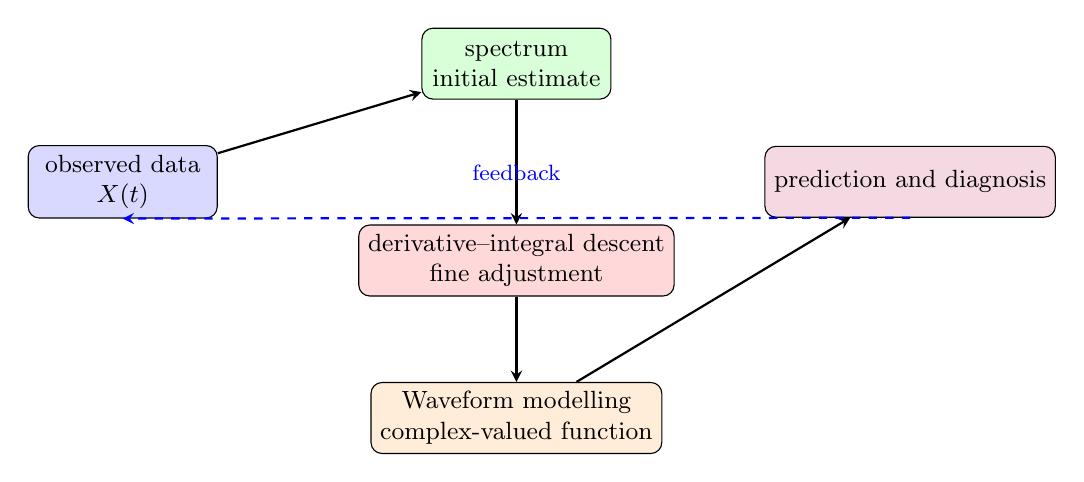
\begin{tikzpicture}[>=stealth,
        box/.style={draw, rounded corners, minimum width=2.4cm, minimum height=0.9cm, align=center, font=\small},
        arrow/.style={->, thick, >=stealth}]
        
        \node[box, fill=blue!15] (data) at (0,0) {observed data\\$X(t)$};
        \node[box, fill=green!15] (fft) at (5,1.5) {spectrum\\initial estimate};
        \node[box, fill=red!15] (kdi) at (5,-1) {derivative--integral descent\\fine adjustment};
        \node[box, fill=orange!15] (waveform) at (5,-3) {Waveform modelling\\complex-valued function};
        \node[box, fill=purple!15] (pred) at (10,0) {prediction and diagnosis};
        
        \draw[arrow] (data) -- (fft);
        \draw[arrow] (fft) -- (kdi);
        \draw[arrow] (kdi) -- (waveform);
        \draw[arrow] (waveform) -- (pred);
        \draw[arrow, dashed, blue, thick] (pred.south) -- node[below, font=\footnotesize, yshift=0.8cm] {feedback} (data.south);
    \end{tikzpicture}
    \caption{Cooperative pipeline of the Waveform and derivative--integral descent.}
    \label{fig:waveform_kdi_pipeline}
\end{figure}

\begin{remark}[Unity with the whole book]\label{rem:methodology_unity}
The modelling and analysis framework established in this chapter is the methodological integration of the whole theory of periodicity mathematics. The core class system takes Functor as its unifying abstraction and is divided into three modules: the function class hierarchy (Functor + basic functions + Epicycle + Waveform + Convolution), the series class hierarchy (Series + Taylor + Fourier + Laurent + Periodic), and the integral transform and sampling classes (Sampler + Sample + Spectrum + Spectral).

The Waveform as the complex-valued function of epicycles is the convergence point of this methodological framework. The joint use of the Waveform, its complex exponential activation-function implementation and derivative--integral descent optimisation makes the complete theoretical system of periodicity mathematics directly applicable to such modern data-science tasks as neural networks, time series analysis and signal processing. Periodic convolution provides a unified operator framework for the interaction between Waveforms.

\textbf{Interface with the next chapter}: the Waveform definition of this chapter (\cref{def:waveform_definition}) and the Epicycle class (\cref{def:epicycle_class}) provide the mathematical object on which the `Epicycle Activation Function and Function Approximation' chapter is based; the CEAF definition (\cref{def:eaf_methodology}) and \cref{def:epicycle-activation} of that chapter are the same mathematical object expressed in two contexts.
\end{remark}

\section*{Seven-theme comparison table for this chapter}

\begin{center}
\renewcommand{\arraystretch}{1.3}
\begin{tabular}{@{}p{2.2cm} p{10.5cm}@{}}
\toprule
Theme & Corresponding content in this chapter \\
\midrule
Translation & The advancement of the time series in data acquisition and dynamic sampling (\cref{def:data_acquisition}); the time-translation invariance of the Waveform (\cref{prop:waveform_properties}(iii)) \\
Scaling & The complexity penalty $K\ln n$ of BIC (\cref{ch34_pipeline_closure}); multi-scale window functions (\cref{def:processing_tools}); the frequency scaling of the Waveform (\cref{prop:waveform_properties}(iv)) \\
Rotation & The phase $\phi_k$ of the epicycle model (\cref{def:epicycle_modelling}); the complex phase representation of the Waveform (\cref{def:waveform_definition}); global phase rotation (\cref{prop:waveform_properties}(v)) \\
Balance & The fit--complexity balance of BIC (\cref{prop:bic_balance}); the parameter uniqueness of the Bohr mean (\cref{ch34_epicycle_properties}(ii)) \\
Symmetry & The hierarchical symmetry of epicycle nesting; the time-translation invariance of the model (\cref{ch34_epicycle_properties}(iii)) \\
Closure & The feedback-iteration closure of the methodological procedure (\cref{ch34_pipeline_closure}); the closure property of the Functor class (\cref{prop:functor_closure}) \\
Period & Spectral peak identification (\cref{def:period_identification}); epicycle parameter estimation (\cref{def:epicycle_modelling}); the convolution closure of the Waveform (\cref{prop:waveform_properties}(ii)) \\
\bottomrule
\end{tabular}
\end{center}

\section*{Exercises}

\begin{enumerate}[leftmargin=3em, label=\textbf{Exercise \arabic*}]
    \item Prove the \textbf{feedback closure of the methodological pipeline} of this chapter (\ref{ch34_pipeline_closure}). Hint: first write down the decision mapping and the evolution group of this chapter's target, then apply the proof structure of the general criterion given in the `Periodic Systems' chapter.

    \item Verify that the hypotheses of the \textbf{derivative closure of basic functions} (\ref{prop:basic_function_derivative_closure}) hold for the domain objects of this chapter, and give a counterexample in which the hypotheses fail.

    \item Examine the behaviour of the \textbf{relation between Series and Waveform} (\ref{prop:series_waveform_relation}) under parameter degeneracy, and explain how the conclusion degenerates accordingly.

    \item Discuss the \textbf{completeness of the modelling steps} as a methodological convention (an \textbf{empirical observation / research programme}; see the remark at \ref{prop:modelling_completeness}) and its relation to the corresponding general conclusion of the `Periodic Systems' chapter (whether it agrees with it, is a special case of it, or requires additional conditions).

    \item Using the seven-theme comparison table of this chapter, identify respectively the concrete carriers of this chapter under the three themes \textbf{translation}, \textbf{scaling} and \textbf{rotation}, and give one example of domain data for each.

    \item Synthesis: restate the diagnostic procedure of this chapter using the five-step standard interface of the `Periodic Systems' chapter (Table \ref{tab:ps_five_steps}), noting one by one the conclusion of this chapter on which each step depends: \ref{ch34_pipeline_closure}, \ref{prop:basic_function_derivative_closure}, \ref{prop:series_waveform_relation}, \ref{prop:modelling_completeness} (an \textbf{empirical observation / research programme}).
\end{enumerate}


